
\documentclass[10pt,a4paper,twoside,openright,fleqn,%
               parskip=half,%
               BCOR=5mm,DIV=10,footinclude=false%
               numbers=noenddot,cleardoublepage=empty]{scrbook}

\usepackage[utf8]{inputenc} 
\usepackage{mathpazo} %-- use Palatino font
\usepackage{amsmath,amssymb,amsthm}
\usepackage[square]{natbib}
\usepackage{subcaption} 
\usepackage{xspace}
\usepackage[breaklinks=true,
            colorlinks=true,
            linktocpage=true,
            allcolors=colorforlinks]{hyperref} 
\usepackage[ruled,vlined,algochapter,linesnumbered]{algorithm2e}
\usepackage{calc}
\usepackage{ccicons} 
\usepackage{xspace} 
\usepackage{booktabs} 
\usepackage[english]{babel}  
\usepackage{listings}
\usepackage{scrhack} % ignore warnings about deprecated KOMA-Script
\usepackage[printonlyused,smaller,withpage]{acronym}
\usepackage[usenames,dvipsnames]{xcolor}
\usepackage{graphicx}
\usepackage{pdfpages}
\usepackage{todonotes}

% [JF] added later by me 
% \usepackage{acro}
% \usepackage{acronym}



\newcommand{\myName}{Jos Feenstra}
\newcommand{\myTitle}{Geofront: Library portability in a browser based visual programming language for geo-computation}

\newcommand{\myGroup}{3D geoinformation group}
\def\myGroupLogo{figs/tud-3dgeoinfo-black.png}
\newcommand{\myUni}{Delft University of Technology}

\newcommand{\myGraduationYear}{2022}
\newcommand{\myGraduationMonth}{June}

\newcommand{\mySupervisorOne}{Ir.\ Stelios Vitalis}
\newcommand{\mySupervisorTwo}{Dr.\ Ken Arroyo Ohori}
\newcommand{\mySupervisorThree}{Dr.\ Giorgio Agugiaro}
\newcommand{\myCoreader}{Dr.\ Hugo Ledoux}

%-- for names for \autoref commands
\def\chapterautorefname{Chapter}
\def\sectionautorefname{Section}
\def\subsectionautorefname{Section}
\def\subsubsectionautorefname{Section}
\def\algorithmautorefname{Algorithm}

% a way to make images fit the paper
% https://tex.stackexchange.com/questions/86350/includegraphics-maximum-width
\def\maxwidth{460pt} 


%-- for pdf metadata
\hypersetup{pdfauthor={\myName}}
\hypersetup{pdfkeywords={thesis, geomatics, TU Delft}}
\hypersetup{pdfsubject={A thesis submitted to the Delft University of Technology in partial fulfillment of the requirements for the degree of Master of Science in Geomatics}}
\hypersetup{pdftitle={\myTitle}}

%-- handy shortcuts
\newcommand{\ie}{i.e.}
\newcommand{\eg}{e.g.}
\newcommand{\reffig}[1]{Figure~\ref{#1}}
\newcommand{\refsec}[1]{Section~\ref{#1}}
\newcommand{\refchap}[1]{Chapter~\ref{#1}}

% [JF]: added a command to prettify this dodgy syntax. m stands for monospace
\newcommand{\m}[1]{\texttt{#1}}

%-- colours for the hyperlinks
\definecolor{colorforlinks}{RGB}{27, 60, 131}

\lstdefinestyle{note}
{
    breaklines=true, 
    basicstyle=\footnotesize,
    keywordstyle=\color{blue},
    commentstyle=\color[rgb]{0.13,0.54,0.13},
    backgroundcolor=\color{cyan!10},
}
\lstnewenvironment{note}
{\lstset{style=note}}
{}

% I keep changing the styling of geofront, so lets put them here
\newcommand{\geofront}{Geofront}

% I keep changing research questions, so lets put them here
% \newcommand{\myMainRQ}{\textit{How to design and implement a web-based vpl for geo-computation which supports running existing geo-computation libraries in a web browser?}}
\newcommand{\myMainRQ}{\textit{How can native geocomputation libraries be \emph{compiled}, \emph{loaded}, and \emph{utilized} within a browser-based dataflow-VPL?}}

\newcommand{\mySubRQOneTitle}{Representation} % previously: facilitation
% \newcommand{\mySubRQOne}{\textit{To what extent is a browser-based application able to facilitate a generic 3D geometry vpl?}}
\newcommand{\mySubRQOne}{\textit{How to implement a browser-based dataflow-vpl for processing 3D geometry?}}

% \newcommand{\mySubRQOne}{\textit{How to implement a visual programming environment in a browser which able to facilitate geo-computation?}}
\newcommand{\mySubRQTwoTitle}{Compilation}
\newcommand{\mySubRQTwo}{\textit{How can geocomputation libraries written in system-level languages be \textbf{compiled} for web consumption?}}
\newcommand{\mySubRQThreeTitle}{Loading}
\newcommand{\mySubRQThree}{\textit{To what extent can a web-consumable library be \textbf{loaded} into a web-vpl without explicit configuration?}}
\newcommand{\mySubRQFourTitle}{Utilization}
% \newcommand{\mySubRQFour}{\textit{What are the advantages and disadvantages of \textbf{using} an existing geoprocessing library through a geo-web-vpl, as opposed to native utilization of said library?}}
\newcommand{\mySubRQFour}{\textit{How can a 'geo-web-vpl' be \textbf{used} to create geodata pipelines?}}








% ********************************************************************
% listings from arsclassica
% ********************************************************************

\let\orgtheindex\theindex
\let\orgendtheindex\endtheindex
\def\theindex{%
	\def\twocolumn{\begin{multicols}{2}}%
	\def\onecolumn{}%
	\clearpage
	\orgtheindex
}
\def\endtheindex{%
	\end{multicols}%
	\orgendtheindex
}

\makeindex

% ********************************************************************
% listings
% ********************************************************************

\definecolor{lightergray}{gray}{0.99}

\lstset{language=[LaTeX]Tex,
    keywordstyle=\color{RoyalBlue},
    basicstyle=\normalfont\ttfamily,
    commentstyle=\color{Emerald}\ttfamily,
    stringstyle=\rmfamily,
    numbers=none,
    numberstyle=\scriptsize,
    stepnumber=5,
    numbersep=8pt,
    showstringspaces=false,
    breaklines=true,
    frameround=ftff,
    frame=lines,
    backgroundcolor=\color{lightergray}
} 

\lstset{morekeywords=%
        {function, f32, i32},
        commentstyle=\color{Emerald}\ttfamily,%
        frame=lines}

\lstset{basicstyle=\normalfont\ttfamily}
\lstset{flexiblecolumns=true}
\lstset{moredelim={[is][\normalfont\itshape]{/*}{*/}}}
\lstset{basicstyle=\normalfont\ttfamily}
\lstset{flexiblecolumns=false}
\lstset{moredelim={[is][\ttfamily]{!?}{?!}}} 
\lstset{escapeinside={£*}{*£}}
\lstset{firstnumber=last}
\lstset{moredelim={[is][\ttfamily]{!?}{?!}}}

\DeclareRobustCommand*{\pacchetto}[1]{{\normalfont\ttfamily#1}%
\index{Pacchetto!#1@\texttt{#1}}%
\index{#1@\texttt{#1}}}

\DeclareRobustCommand*{\bibtex}{\textsc{Bib}\TeX%
\index{bibtex@\textsc{Bib}\protect\TeX}%
}

\DeclareRobustCommand*{\amseuler}{\protect\AmS{} Euler%
\index{AmS Euler@\protect\AmS~Euler}%
\index{Font!AmS Euler@\protect\AmS~Euler}}

\lstnewenvironment{code}% 
{\setkeys{lst}{columns=fullflexible,keepspaces=true}%
\lstset{basicstyle=\small\ttfamily}%
}{}

\lstset{extendedchars} 
\lstnewenvironment{sidebyside}{% 
    \global\let\lst@intname\@empty 
    \setbox\z@=\hbox\bgroup 
    \setkeys{lst}{columns=fullflexible,% 
    linewidth=0.45\linewidth,keepspaces=true,%
    breaklines=true,% 
    breakindent=0pt,%
    boxpos=t,%
    basicstyle=\small\ttfamily
}% 
    \lst@BeginAlsoWriteFile{\jobname.tmp}% 
}{% 
    \lst@EndWriteFile\egroup 
        \begin{center}% 
            \begin{minipage}{0.45\linewidth}% 
                \hbox to\linewidth{\box\z@\hss} 
            \end{minipage}% 
            \qquad 
            \begin{minipage}{0.45\linewidth}%
            \setkeys{lst}{frame=none}% 
                \leavevmode \catcode`\^^M=5\relax 
                \small\input{\jobname.tmp}% 
            \end{minipage}% 
        \end{center}% 
} 

\lstset{numbers=left,
    numberstyle=\scriptsize,
    stepnumber=1,
    numbersep=8pt
}   

\setcapindent{1em} %-- for captions of Figures
% \setcounter{tocdepth}{\sectiontocdepth}

\subject{MSc thesis in Geomatics}
\title{\myTitle}
\author{\myName}
\date{\myGraduationMonth\xspace\myGraduationYear}
\publishers{A thesis submitted to the Delft University of Technology in partial fulfillment of the requirements for the degree of Master of Science in Geomatics}

\begin{document}


%******************************************************************
% Frontmatter
%******************************************************************
\frontmatter

%******************************************************************
% The cover page 
% (it needs to be manually edited and exported as a PDF)
% (see folder README.txt in folder 'cover')
% (I would not include it for the version you put in the repository)
%******************************************************************

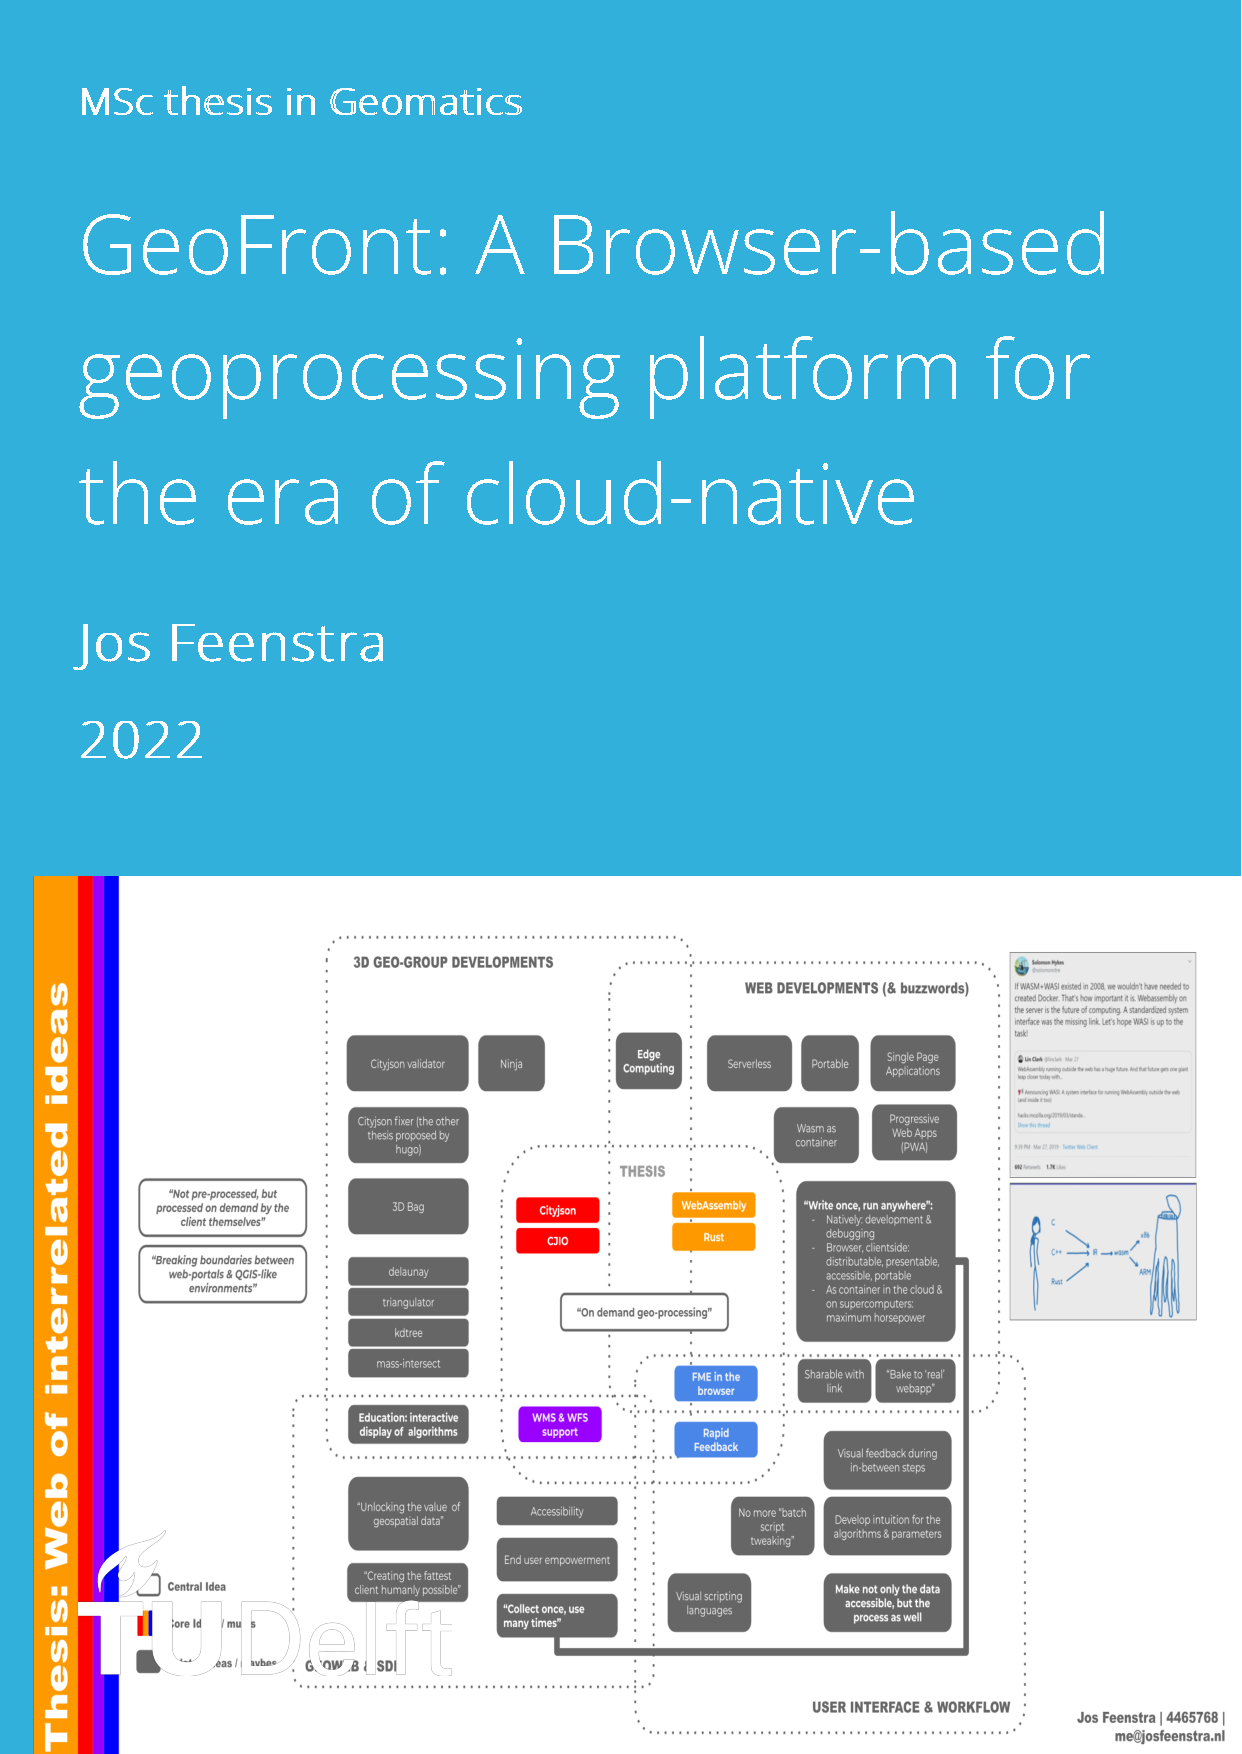
\includepdf{0-cover/cover_front.pdf}
\cleardoublepage

\maketitle[3]

% \clearpage
%!TEX root = ../thesis.tex

\thispagestyle{empty}

\hfill
\vfill

\noindent\myName: \textit{\myTitle} (\myGraduationYear)\\
\ccby\xspace This work is licensed under a Creative Commons Attribution 4.0 International License. To view a copy of this license, visit \url{http://creativecommons.org/licenses/by/4.0/}.

\vspace{3em}


\vspace{3em}

\noindent{} The work in this thesis was carried out in the:\\

\begin{tabular}{ll}
\parbox{0.3\textwidth}{\includegraphics[width=\linewidth]{\myGroupLogo}}
&
\parbox{0.7\textwidth}
{
  \myGroup\\
  \myUni\\
}       
\end{tabular}

\vspace{3em}
\noindent
\begin{tabular}{ll}
Supervisors:  &  \mySupervisorOne \\
              &  \mySupervisorTwo \\
Co-reader:    &  \myCoreader\\
\end{tabular}


\cleardoublepage
\chapter*{Abstract}

X is an essential part of any ...

The problem ...

The goal of this study is to

This study presents and prototypes a novel method which allows \ac{GIS} practitioners without a background in software development, to access the full potential of core transformation and analysis capabilities found in native \ac{GIS} libraries.

% That is based on visual programming, and static web applications. 


% The study attempts to meet this goal by designing and implementing a 
novel method based on the fields of visual programming, and static web applications. 

% The prior works on static geo-web applications and \ac{GIS} \ac{VPL}s indicate that a strong theoretical framework is in place.
% But, and this is especially evident in the prior studies regarding Browser-based geocomputation, the practical implementation of these theories were only partially successful, and limited in scope. 
% This necessitates a practical approach in response. 

A Prototype VPL was developed to host the functionalities of \ac{GIS} libraries from within an application, and in a composable manner. Additionally, it is used to connect these libraries to various \ac{GUI} features. 
The format of web application is used to allow this prototype to be directly accessible to end users without installation or configuration. 
% Geodata used within the application is also exclusively statically hosted geodata, or user-submitted data. 
This prototype is statically hosted, to minimize operational costs, and is equipped with WebAssembly, so that libraries written in native languages can be used without resorting to active backend web services. 
Finally, as this prototype is intended for \ac{GIS} usage, both scalability to handle sizable datasets, and rich \ac{GUI} support (3D viewers, file inputs, sliders, text boxes, graphs), are primary design considerations and assessment criteria.

Using this, ...

This method turned out to indeed provide solve

The significance of this method lies herein that it ...


% This method is thereafter used to load various \ac{GIS} libraries, and used in demo applications, after which an assessment can be made on its quality and the extend of its achieved functionalities. 
% The study concludes by addressing if the method meets the overarching goal.


% Geocomputation is a cornerstone of GIS \& modern mapping needs.
% While the last decades have seen major advancements, writing a geocomputational pipeline remains a complex, non-trivial exercise. 
% Performing geocomputations by utilizing a visual programming language (VPL) within a web browser is a novel development which seeks to simplify this process, allowing more people to write these types of pipelines more successfully.
% It would, in theory, allow end-users to author geocomputation pipelines, without the need of a software development background, and without the need to install software.
% utilizing a dataflow model.
% This model is the standard within VPLs dealing with geometry processing, and contains many advantages in terms of performance and reliability.

% In this context, the portability of existing geocomputation libraries is a common problem.
% This is often addressed by maintaining duplicate JavaScript alternatives to libraries such as GDAL, PROJ, and GEOS, complicating innovation.  

% This study seeks to improve the state of browser-based geocomputation VPLs by attempting to bring industry-standard geo-libraries to these environments. 
% The study poses that this can only be done if native geocomputation libraries can be \emph{compiled} to WebAssembly, \emph{loaded} into a VPL, and \emph{utilized} in a browser-based dataflow-VPL format.
% Discovering if and how these steps can be performed is the central question of this study. 
% % This study seeks to improve the state of web-based geocomputation VPLs 
% % by discovering if the library portability problem can be overcome, and if so, how.

% This question is answered by testing a possible solution.
% A proof of concept web-based VPL is designed, implemented and evaluated, which makes use of a novel plugin system, as well as a directed, acyclic graph-based data model \& interface.

% Using this proof of concept, the study was able to demonstrate that the web platform was sufficiently capable of representing a dataflow VPL capable of constructing geocomputation pipelines.
% The functional programming-properties of this dataflow VPL also makes geo-libraries sufficiently \emph{usable}, albeit with some well-known caveats of dataflow-VPLs, like the representation of conditionals and iteration.  

% The current methods of \emph{compiling} existing C++ geocomputation libraries to the web turned out to be insufficient for the purposes of this study.  
% This is due to the Emscripten compiler's focus on compiling full C++ applications instead of separate libraries. 
% Despite this, the study wás able to demonstrate how a novel method can be used to sufficiently \emph{compile} and \emph{load} multiple Rust-libraries for usage in the VPL, thanks to more feature-rich WebAssembly tools in the Rust ecosystem. 
% While Rusts geocomputation libraries are young, the study presents this method to either offer emscripten contributors a blueprint of a desired workflow, or to offer geocomputation library contributors a powerful use-case for the Rust language. 

% All in all, this means that either if the geocomputation libraries found in the Rust ecosystem mature, or if Emscripten's capabilities improve, then the code portability problem \& dataflow problem of existing web-based geocomputation VPLS can be solved. 


% \begin{note}

%     "make a simple narrative of what you did and what are the results."
%     "make it not be a very rough draft"
%     "6.2: deliver the things you promised."
%     "make it more formal: replace: "crucial", "by far" or "impressive""

%     Stelios Draft Comments
%     ======================
    
%     In general, I think it's going well. I think the intro is fine, although it can be improved. I like the conclusions quite a lot, tbh. You are giving proper and interesting answers to the raised questions. The rest is a bit of a very rough draft, as I see. So, some specific points:
    
%     TODO: Tone down stuff
%     -  It seems like you have placed several bits here and there that seem like either introduction or conclusions. I feel your enthusiasm and excitement in your writing, but I think you are bringing questions and answers in places were people would normally just expect a simple narrative of what you did and what are the results.
    
%     TODO: Write 6.2
%     -  Speaking of results, we are missing the experiments so please put this at your first priority. This is because it feels like you promise things that you do not deliver.
    
%     TODO: Find & Replace
%     -  In general, you are using some very bold statements and informal expressions. The latter is kinda okay, but the first one is very dangerous. I've noticed words like "crucial", "by far" or "impressive" which seem very biased and subjective, so better be avoided. You can still use them here and there (mostly in the conclusions), but I think you use them way  too much (again, I can see your enthusiasm).
    
%     TODO: Find & Replace 
%     -  Minor thing, but I think you have confused \citet with \citep. The first one is used when the citation is part of the sentence and the latter when it's at the end of a sentence (or in a parenthesis, anyway).
    
% \end{note}

% This might allow web based VPLs for geocomputation to be 
% Geodata computation is important.
% Geodata computation is difficult.
% geo-web-vpls could help, but have seen little research
% This study: design, implement, analyze a new prototype geo-web-vpl. 
% Design-> utilize existing, native libraries written in C++ \& Rust on the web, in the format of a vpl.

% results -> it works.

% -> study shows that interplay between textual and visual programming is possible


% \begin{note}
%  - Performance intensive: (Big data, O(n^2) problems) 
%  - Heterogenous data (type, quality, scale, criteria, crs) 
%  - Complex (geometric) operations (linalg, bundle adjustment, procedural modelling) 
% \end{note}

% All of this makes the process of geocomputation difficult. 


% The full flowchart runs client-side in a browser, and both end results and intermediate products can be inspected in a 3D viewer.

% GeoFront offers several functionalities such as the parametric creation of 2D and 3D primitives, triangulation, isocurve extraction, and more. 
% These functionalities can be expanded upon though a plugin system which utilizes the existing "Node Package Manager" infrastructure.
% Together with WebAssembly, this enables the utilization of industry standard geoprocessing libraries such as `CGAL`, `GDAL` and `PROJ`, and data parsing libraries such as `IFC.js` and `laz-rs`.



% Following the implementation, the project was tested by simulating use-case scenarios. 
% The tests demonstrate the feasibility of [...]
% At the same time some key parameters of [...] identified which if tuned properly they can optimize the performance, behavior and robustness of the geo-web-vpl.
% With the project being a prototype solution, the vpl is far from operational and there is certainly a lot of space for improvement regarding both components. 

% 1. Tryout (ACTUAL)
%    - A-la wapm WebAssembly Package Manager allows packages to be run from within the package-page itself. 
%   - Just meant to quickly try out some features.

% 2. Educational (ACTUAL)
%    - interactive educational tool
%    - (What does a delaunay triangulation look like? how does it behave? What happens if you lower the radius of inverse distance weighting ? )

% 3. Rapid-Prototyping (POSSIBLE)
%    - Setting up pipelines which can be consumed by cloud-based geoprocessing services. 
%    - Future work: export flowchart to a process which can be run natively or server side.

% 4. Publishing (POSSIBLE)
%    - Geotiff.io / ModelLab
%    - Web FME 
%    - Publish full web apps in and off themselves, making use of zero, one or multiple wasm-compiled libraries.  
%    - Future work: export to web-app (without flowchart)

% % Safesoft's FME, but web based \& open source 

% % CONCLUSION
% By creating geofront, this thesis was able to discover .............

% - The web is able to facilitate a visual proregramming language.

% - The web is able to be used for geoprocessing, albeit with some caveats
%   - TypedArrays,
%   - Geometric predicates 
%   - Rounding
%   - ETC.

% - Many of these things can be fixed with webassembly, but webassembly itself has other shortcomings
%   - Differences between Rust \& C++

% - reasonable performance 
%   (- great considering the platform)

% - would not be possible without these modern web features
%   - Web Assembly 
%   - Typed Array's 
%   - Web Workers
%   - Web Components,
%   - 2D Canvas API
%   - Web GL

% \todo{[JF]: I need to add more critical notes on promises of accessibility. Is a webapp truly accessible? Is a flowchart interactive, or does it hinder interactiveness? }

% I believe that such a web application can make geoprocessing more accessible to practitioners.
% This empowers users to create small geoprocessing demo's, and share these 
% With geofront, geoprocessing libraries can be loaded and used interactively. Users are also able to create and share flowcharts.
%%%%%%%%%%%%%%%%%%%%%%%%%%%%%%%%%%%%%%%%%%%%%%%%%%%%%%%%%%%%%%%%%%%%%%

% 


%%%%%



\begin{note}

  Lessons
  ==========
  
  - give yourself clear todo's per day. 
    Not too little, not too much.
    Upon completion, the day falls apart
  
  
  TODO
  ============
  
  high-level
  ----------
  
  [x] The intro / story needs to be altered 
      - stronger tie to Geo & web
      - VPL + Web
  
  [x] rewrite and balance research questions
  - [x] then trickle down the consequences of those changes throughout the thesis
  mid-level
  ---------
  
  [ ] TODO: rewrite abstract in accordance with new story

  [x] Deep dive in Hugo's comments, fix those aspects 
    - [x] sort acronyms
  
  [x] Add a stronger web-component in the introduction (presentation)
  [x] Add cloud native / cloud-based geodata component to the introduction  
  
  [ ] Cleanup Chapter 2 and 3.  
    - Some parts are still more relevant than other parts. 
    - Also, there are some things I say or use in chapter 4, 5, and 6, that were not properly explained in chapter 2. Examples of this are emscripten, or CGAL. 
    - However, a complete rewrite would be too much work.
    - Would love to hear your take on this.
  
  [ ] Make chapter 4 and 5 more streamlined 
    - I've noticed that I repeat myself quite often.
    - I think this is because I was not sure if I already said something relevant in the chapter before.
  
  [ ] Show your results more clearly, do the coding you have done justice
  
  [ ] finish chapter 6 properly 
    - Experiments: add a section on a use-case application, using potree + startin + geofront std + obj downloader
  
  [x] write stronger, more clear conclusions.
    - hmm, i think they are already quite clear. But again, this is to be reconsidered when the overall story of the thesis changes  
  
  low-level: thursday & friday
  -------------------

  - [ ] write 
  - [x] TODO: write Acknowledgements
  - [x] Add arsclassica template to the thesis
  - [x] Make the code snippets / listings work properly
  - [x] replace all code screenshot with proper listings
  - [ ] create all missing uml diagrams
  - [ ] add proper graphs for the data you've gathered 
  - [ ] Add all proper metadata to Zotero, for a nice bibliography
  - [ ] Fix all TODO graphics
  - [ ] Fix all acronyms,
  - [ ] Sort the acronyms at the end 
  - [ ] Make sure CiteT and citeP is properly used everywhere. No more raw 'et. al.' statments 
  - [ ] Capitalize all VPL / replace with acronyms
  - [ ] Sources need to be fixed (more data, check if I can do things like 'empscripten contributors')
  - [ ] Replace C++ into C / C++ everywhere, but especially the intro
  - [ ] appendix: software implementation & link to video
\end{note}


\chapter*{Acknowledgements}

\begin{itemize}
    \item Stelios
    \item Ken
    \item Martin, Current employer, GeoDelta 
    \item Sybren, Previous employer, Sfered
    \item Nadja
    \item Tim
    \item Friends \& Family
\end{itemize}

\ldots



 
\clearpage

\setcounter{tocdepth}{2}

\tableofcontents
\listoffigures
% \listoftables
% \listofalgorithms


\clearpage
\chapter*{Acronyms}

% thank you, vscode sort lines extension!
\begin{acronym}
    \acro{CDN}{Content Delivery Network}
    \acro{CGAL}{Computational Geometry Algorithms Library}
    \acro{CLI}{Command Line Interface}
    \acro{CRS}{Coordinate Reference System}
    \acro{DAG}{Directed Acyclic Graph}
    \acro{DEM}{Digital Elevation Model}
    \acro{DT}{Delaunay triangulation}
    \acro{DTM}{Digital Terrain Model}
    \acro{DSM}{Digital Surface Model}
    \acro{ETL}{Extract Transform Load}
    \acro{EUD}{End User Development}
    \acro{FOSS}{Free and Open Source Software}
    \acro{GDAL}{Geospatial Data Abstraction Library}
    \acro{geo-vpl}{geocomputation or geometry VPL}
    \acro{geocomputation}{Geospatial data computation}
    \acro{GEOS}{Geometry Engine Open Source}
    \acro{GIS}{Geographical Information Science}
    \acro{GUI}{Graphical User Interface}
    \acro{HTTP}{Hyper Text Transfer Protocol}
    \acro{IDE}{Integrated Development Environment}
    \acro{MVC}{Model View Controller}
    \acro{os}{operating system}
    \acro{OSGEO}{Open Source Geospatial Foundation}
    \acro{OGC}{Open Geospatial Consortium}
    \acro{TIN}{triangular irregular network}
    \acro{UI}{User Interface}
    \acro{UX}{User Experience}
    \acro{VD}{Voronoi diagram}
    \acro{VPL}{Visual Programming Language}
    \acro{W3C}{World Wide Web Consortium}
    \acro{wasm}{WebAssembly}
    \acro{WFS}{Web Feature Service}
    \acro{WMS}{Web Mapping Service}
    \acro{WPS}{Web Processing Service}
    % \acro{etl}{Extract Load Transform}
\end{acronym}


% WHY DOESNT THIS SHOW UP???
% https://tex.stackexchange.com/questions/557187/acronyms-in-a-table-environment-are-not-shown-in-the-list-of-acronyms


\cleardoublepage

%******************************************************************
% Mainmatter
%******************************************************************
\mainmatter

%-------------------------------------------------------------------------------------------------%
% An introduction in which the relevance of the project and its place in the 
% context of geomatics is described, along with a clearly-defined problem statement.
% [KEN]
% instead, I think you can start by saying that web applications are popular
% explain the benefits briefly
% apart from having no installation

% then, I think you can make a better argument for your thesis overall
% explain that historically, thin client fat server was the standard
% for the reasons you listed
% and then directly explain why this is potentially changing now

\newpage
\section{Introduction}

% Dissolving the discrepancy between visualization \& processing in web-apps.

% web is popular 
% geoweb-applications are popular 
% online geodata processing is popular 
% client-side geodata processing 


% STELIOS: Relatively slow
 
% show an example 

Interactive, browser-based \ac{gis} applications form an indispensable component of the modern geospatial software landscape. A web application is cross-platform in nature, and offers ease of maintainability and access, since no installment or app-store interaction is required to update or run the app. The ability be placed as a supplement within the larger context of a webpage is also not trivial. These features have made the browser a popular host for many \ac{gis} applications, especially when targeting end-users. 

% streamline these three paragraphs.
% I want something like -> problem: limitations. 

Despite the popularity of \ac{gis} web applications, the range of actual \ac{gis} abilities these applications are capable of is very limited. For example, \ac{geoprocessing}, like CRS translations, interpolation, boolean operations, or raster transformation kernels are usually not present within the same software environment as the web app. This limited range of capabilities limits the usefulness of \ac{gis} web applications, and with it the number of use cases a \ac{gis} web application can serve. Current geospatial web applications serve for the most part only as lightweight viewers; visualizers of pre-processed data. If web applications gain these functionalities, they could grow to be just as diverse and useful as desktop \ac{gis} applications. It would allow for a new range of interactive web applications, in which data users can post-process geodata quickly, uniquely, and on demand.

This raises the question of Why. Why are web \ac{gis} applications limited to just be viewers?

% This raises the question: why is this not done yet? two reasons 
% 1. People are content with server-side geoprocessing 
%    -> BUT: this does not serve every use-case 
% 2. Client-side geoprocessing is hindered by javascript and the web environment
%    -> NOT ANYMORE: WebAssembly
% 
% 
% To solve 2: WebAssembly
% To solve 1: We offer a case study which demonstrates a unique type of application which would not be possible without client-side geoprocessing. 

However, by making the functionality of an application not self-contained but distributed, 

The improvements of client-side hardware have opened up a second possibility: client-side geoprocessing, directly within a web application. By doing this, the hard divide between client visualization and server processing could be bridged.  while at the same time driving down the operational costs of geoprocessing servers. This is why client-side \ac{geoprocessing} in web applications is slowly gaining traction during the last decade \cite{kulawiak_analysis_2019, panidi_hybrid_2015, hamilton_client-side_2014}. 

% Interactive geospatial data manipulation and online geospatial data processing techniques are described as "current highly valuable trends in evolution of the Web mapping and Web GIS" \cite{panidi_hybrid_2015}. 

However, serious drawbacks to client-side geoprocessing where encountered during these studies. Browser-based geoprocessing suffers from the fact that it will need to be written in the `JavaScript` programming language. Previous attempts at client-side geoprocessing have shown that JavaScript based geoprocessing libraries do not offer the performance required for proper geodata processing \cite{hamilton_client-side_2014}. 
Moreover, the JavaScript library ecosystem does not offer viable alternatives to industry-standard libraries like CGAL and GDAL. 
% This would require alternatives to be rewritten in JavaScript, or would require the source code of mature libraries to be compiled to JavaScript. Both these solutions would be difficult to maintain, and would still end 
% Both these solutions contain many imperfections. The first option would be an inefficient, time-consuming task, and would mean code duplication. 
% The second option would mean taking C++-based libraries such as CGAL, and compiling them to a special, fast subset of JavaScript called `asm.js` using the `emscripten` compiler \cite{zakai_emscripten_2011}. 
% While this is more fast and reliable, it contains its own set of problems. 
% The generated, rather large JavaScript files usually take a long time to download, to scan, and to be properly optimized by a JavaScript Just In Time (JIT) Compiler \cite{haas_bringing_2017}. 

An emergent technology poses a solution to both problems. At the end of 2019, the \ac{w3c} officially pronounced WebAssembly as the fourth programming language of the web \cite{w3c_world_2019}. Since then, all major browsers have added official WebAssembly support. \ac{wasm} is a binary compilation target meant to be small, fast, containerized, and platform \& source independent \cite{haas_bringing_2017}. \ac{wasm} surpasses javascript in almost all performance aspects: it loads quicker, it is scanned quicker, and since it is close to bytecode, it can often run at a speed comparable to system level programming languages like C++ and Rust \cite{jangda_not_2019}. 

% \cite{beilschmidt_vat_2017}


% Related studies concerned with the performance of WebAssembly, together with the existing software around WebAssembly, pose enough evidence to suggest  theoretically possible (SOURCE: Emscriptem). 
% However, this leaves the question whether it is practically possible unanswered, evident by the fact that no wasm-powered geoprocessing tools exists at the time of writing this study. 

\newpage

% stelios: Speed up 

\subsection{Problem}

If WebAssembly performs as described by \cite{haas_bringing_2017} and \cite{jangda_not_2019}, it could theoretically be the missing link to make client-side geoprocessing viable. However, no wasm-powered geoprocessing tools exists yet at the time of writing. Hypothetically, this is because of two reasons. Firstly, WebAssembly brings along many practical uncertainties:

\begin{itemize}
  \item Do geoprocessing libraries directly compile into WebAssembly? If not, which workarounds are needed? 
  \item Will a \ac{wagl} load efficiently, or should they be split up into parts, and loaded lazily? 
  \item How well do \ac{wagl} operations perform in a browser, compared to their native counterparts? What can be done to make this difference as small as possible?
\end{itemize}

Secondly, the way geoprocessing is supposed to be performed within the context of a web-browser remains unknown. The above list of implementation considerations cover only how \ac{wagl}'s can be \emph{run}. Potential answers do not indicate how \ac{wagl}'s can be \emph{used}. \cite{jangda_not_2019} warns against assessing WebAssembly in a vacuum, and notes how its performance is highly dependent on the way it is used, and the context in which it is used. This context of geoprocessing within a web-browser brings up many considerations as well: 

\begin{itemize}
  \item How will users upload or specify the input in a web-browser?
  \item Can the transformations offered by \ac{wagl}'s be used like functions? Or do they require special services, such as a wrapper library, virtual file system, or a virtual Command line interface? 
  \item How can users recieve and evaluate the output in a web-browser?
  \item How can a sequence of geoprocessing steps be chained together in a web-browser?
  \item How can a web-based \ac{ui} or \ac{gui} facilitate all these functionalities?
\end{itemize}

These two sets of unknowns are highly dependent upon each other. Together, they form a barrier preventing further development of client-side geoprocessing. Since no wasm-powered, client-side geoprocessing application exist yet, there is no way to answer these questions, and no way to confirm the theoretical benefits of WebAssembly for client-side geoprocessing, and the geospatial community at large.



\subsection{Use Case}
% mini methodolody??


in order to demonstrate 

visual programming language.




%-------------------------------------------------------------------------------------------------%
\newpage

%-------------------------------------------------------------------------------------------------%
\subsection{Research Questions}

This study intends to discover if contemporary web technologies can facilitate client-side geoprocessing by seeking an answer to the following question:  

\textit{How to \textbf{design and create} a browser-based GIS environment which can \textbf{effectively utilize} \textbf{existing geoprocessing libraries}, using only the \textbf{current state} of \textbf{standard client-side web technologies}?}

\subsubsection*{Explanation}

% The research question is written purposefully written in the "how well does X support Y question" shape. To unpack its components: 

- \textbf{design and create}: The wording 'design and create' is used to signal that this will consider the theoretical design , as well as the practicalities of creating this design. 

- \textbf{Standard client-side web technologies}: This phrase is meant to limit the scope to only the standard, core technologies of major browsers (Chrome, Edge, Safari, Firefox). This means the four languages \ac{wasm}, CSS, JavaScript and HTML. Additionally, HTML5 gives us WebGl, the 2d Canvas API, SVG's, and Web Components to work with.

- \textbf{Current state}: The study will use contemporary, even bleeding edge features of the modern web, but its findings will nonetheless be bound to this time of writing, as web technologies in particular quickly change. 

- \textbf{Existing geoprocessing libraries}. This wording expresses this studies desire to explore the usage of existing geoprocessing libraries, rather than to recreate geoprocessing libraries from scratch.

- \textbf{Effectively utilize}: The study intends to not only find out how \ac{wagl}'s can be \textit{run} in a browser, but also how \ac{wagl}'s can be \textit{used}. 


\subsubsection*{Sub Questions}

The following sub-research questions are needed in order to answer the main question. The methodology chapter will explain the choices of these sub-questions. 

\textit{1 : What is the most fitting methodology of compiling C++ geoprocessing libraries to WebAssembly?}

\textit{2 : How to design and create a client-side geoprocessing interface for data-users?}

\textit{3 : How can wasm-compiled geoprocessing libraries be distributed and used in a client-side geoprocessing interface?}

\textit{4 : What are the advantages and disadvantages of GIS applications created using a client-side geoprocessing environment powered by WebAssembly?}

\newpage
\subsubsection*{Assessment}

At the final conclusion of the proposed thesis, we can answer if the designed and created GIS environment can indeed effectively utilize these geo-libraries.
this will be answered by quantitative and qualitative means:

Quantity
\begin{itemize}
    \item Have all required features been implemented?
    \item Which libraries can be used?
    \item What are the load \& run times of these libraries, compared to native execution?
\end{itemize} 

Quality
\begin{itemize}
    \item Have all design goals been met?
    \item Can data users 'effectively' handle input, process and output?
    \item Can the load \& run times be regarded as acceptable to use? 
\end{itemize} 


% ----
\subsection{Scope}


\subsection*{Will Include}

The 'will include' scope is represented by the Methodology chapter. 

%-----------------------------------------------------------------------------%
\subsection*{Will not include}

\subsubsection*{Server-side or Native WebAssembly} % **Client-side WebAssembly Only**

This study will limit itself to the \emph{client-side} usage of WebAssembly. 
A powerful case can be made for \emph{server-side}, or native level usage of WebAssembly, especially in conjunction with a programming language such as Rust. 
Rust compiled to WebAssembly could, compared to using python, java or C++, make geoprocessing more maintainable and reliable, while at the same time ensuring memory safety, security, and performance \cite{clack_standardizing_2019}. 

Server-side or native wasm is beyond the scope of this paper, but would be an excellent starting point for future work. Note that this also means that research into \ac{wagl}'s is important for more than just client-side geoprocessing. All geoprocessing could benefit from it.



\subsubsection*{Web Processing Service} % Will not be dealing with WPS 

% offered as server-side geoprocessing services.  
Similarly, this study will exclude the OGC standard of the \ac{wps} \cite{ogc_web_2015}, since these services do not offer \emph{client} side geoprocessing, but instead offer \emph{server} side geoprocessing. A client-side application \textit{could} create an interface to use such a service, to essentially offer geoprocessing to clients, but this study regards a solution like that as a workaround, not a true solution to the problem of client-side geoprocessing. 

This is not to say that client-side geoprocessing replaces the need for \ac{wps}. 
future work could research the possibility of utilizing a hybrid strategy of both client-side and server-side geoprocessing, following in the footsteps of \cite{panidi_hybrid_2015}. 

% Still, We must briefly discuss the \ac{wps}, since it seems to offer a solution to the problems addressed.

%The OGC standard of the \ac{wps} offers a set of protocols to standardize geoprocessing on a server. By specifying input data and instructions to one of these services, polling the status of the process, and then downloading the results once finished, a user can process geodata on a server. If a client-side application creates an interface to use such a service, it can essentially offer client-side geoprocessing.

% While this is more like a workaround for client-side geoprocessing than a solution, it can nonetheless be preferred. A Web Processing Service is an excellent solution when client-side hardware is limited, and when server-side resources are abundant. It is also more efficient if the datasets required for geoprocessing are already located on these servers, and when working with geo-datasets too large to store locally. 

% situational cuts both ways 

% a \ac{wps} do not replace the need for client-side geoprocessing, for much of the same reasons a \ac{wps} does not replace the need for native \ac{gis} applications like QGIS or ArcGIS.  

% The usefulness of a \ac{wps} is, just like client-side geoprocessing, situational. 

% For much of the same reasons \ac{wps} does not replace the 


% reasoning from the perspective of client-side geoprocessing, a \ac{wps} does not offer a true solution to the problem of client-side geoprocessing, but only a workaround. 


% When the reverse is true however, and when the application needs to remain interactive and responsive, other solutions are required.

% While 

% Future work could research the possibility of utilizing a hybrid strategy of both client-side and server-side geoprocessing, following in the footsteps of \cite{panidi_hybrid_2015}. 


\subsubsection*{Usability Analysis} % 

While usability is a major component of this research, no claims will be made that the developed use-case is more usable to native GIS applications or geoprocessing methods. This research attempts to solve practical inhibitions in order to discover whether or not client-side is \emph{an} usable option. If it turns out that this method is viable technically, future research will be needed to definitively proof \emph{how} usable it is compared to all other existing methods.  

% This paper seeks to first close this gap, limiting itself to overcoming the technical and design boundaries in the pursuit of practical client-side geoprocessing.

Similarly, a survey analyzing how users experience client-side geoprocessing in comparison to native geoprocessing must also be left to subsequent research. While this would gain us tremendous insight, client-side geoprocessing is too new to make a balanced comparison. Native environments like GRASSGIS, QGIS, FME or ArcGIS simply have a twenty year lead in research and development. 

%-------------------------------------------------------------------------------------------------%
% A related work section in which the relevant literature is presented and 
% linked to the project. 
% It should show that you clearly know the problem you plan to solve, 
% and that you master the related work. 
\newpage

\section{Related work}

This chapter offers background literature on the aforementioned topics, and will explain how this literature relates to the proposed study. three related topics are regarded: prior studies on WebAssembly, Prior studies on client-side geoprocessing, and prior studies on geoprocessing interfaces.


\subsection{WebAssembly \& Geoprocessing performance}

% Why are you writing this? 

On 5 December 2019, the \ac{w3c} officially pronounced WebAssembly as the fourth programming language of the web \cite{w3c_world_2019}. Philippe Le Hégaret, the \ac{w3c} Project Lead, writes “The arrival of WebAssembly expands the range of applications that can be achieved by simply using Open Web Platform technologies. In a world where machine learning and Artificial Intelligence become more and more common, it is important to enable high performance applications on the Web, without compromising the safety of the users,”. Since then, most major browsers have added WebAssembly support.

To the best of the author's knowledge, and as of writing this proposal, no papers explicitly links WebAssembly and Geodata processing. The original paper paper on \ac{wasm} does state \textit{3d data processing} as one of the examples for high performance web applications \cite{haas_bringing_2017}.. What's more, Google Earth uses WebAssembly as seen in \reffig{fig:google-earth} \cite{google_google_2020}. How it is used is unknown due to the engine being closed-source, but it is speculated that \ac{wasm} is used to access code written for the original C++-based desktop application.


\cite{jangda_not_2019, haas_bringing_2017}.

\begin{figure}[!tbp]
  \centering
  \begin{minipage}[b]{0.80\textwidth}
    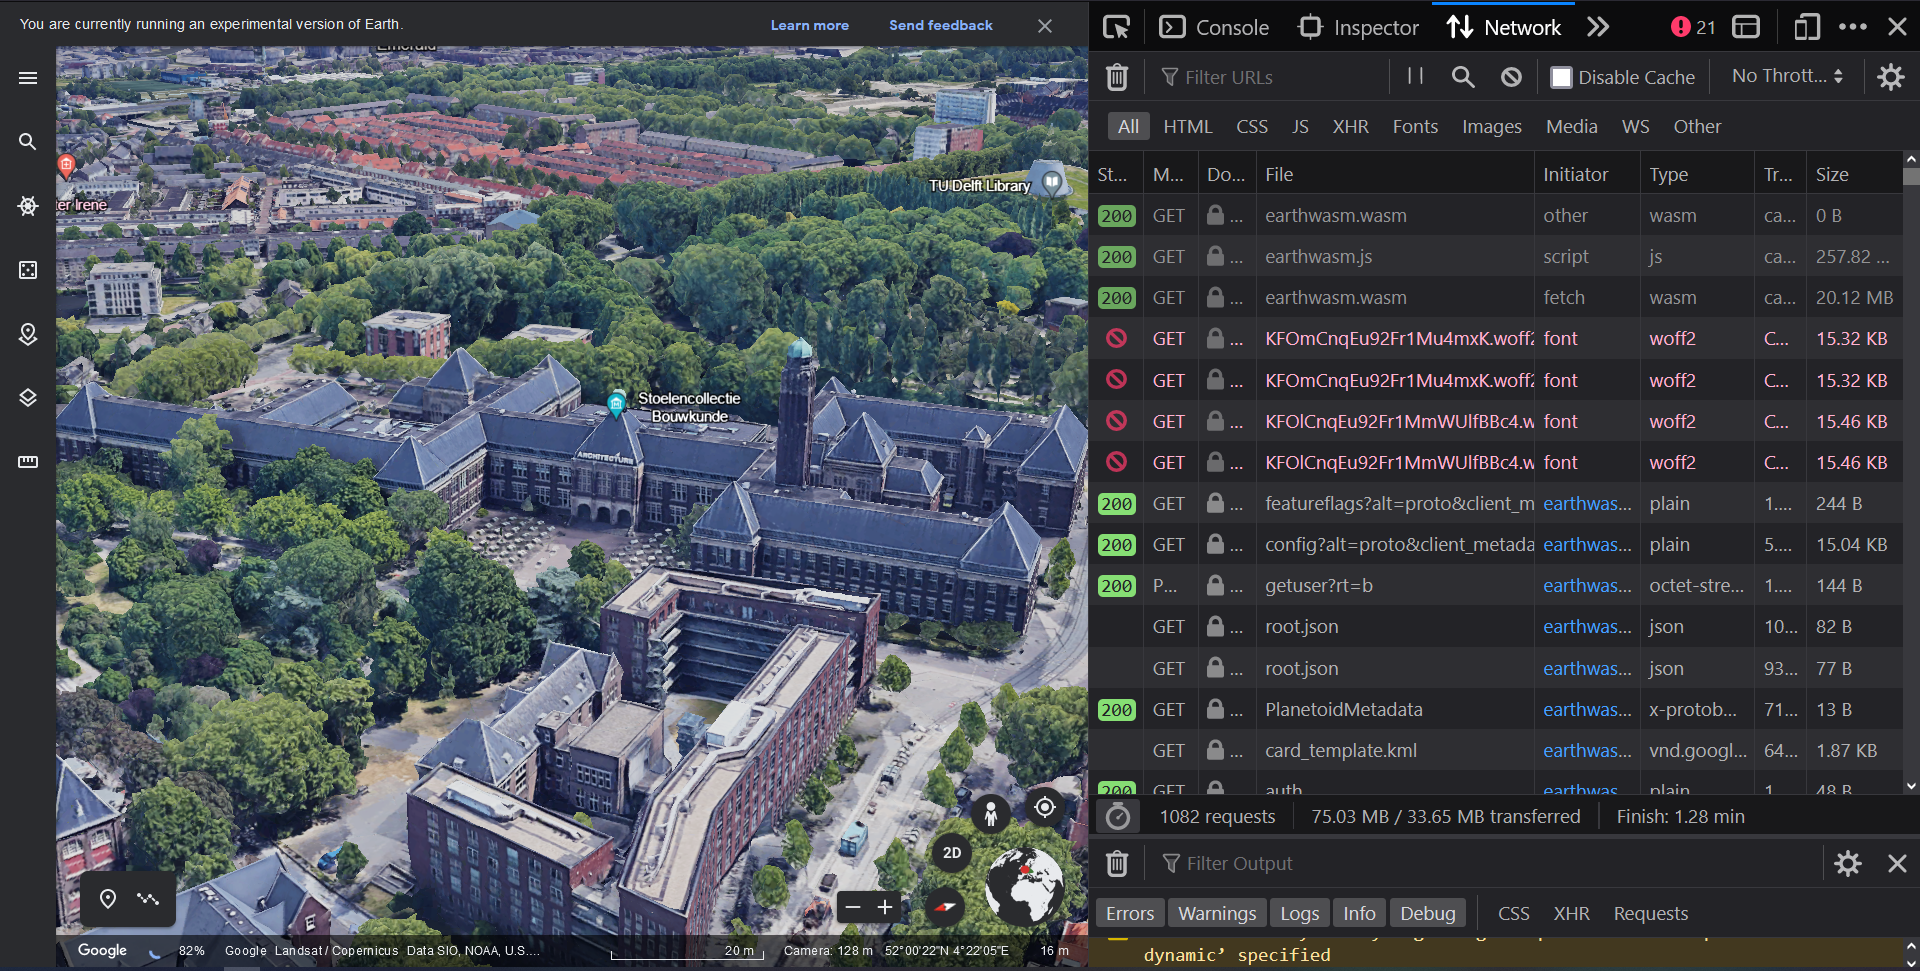
\includegraphics[width=\textwidth]{../images/google-earth-uses-webassembly.PNG}
    \caption{Google Earth utilizing WebAssembly. Source: \cite{google_google_2020}}
    \label{fig:google-earth}
  \end{minipage}
\end{figure}



The performance benefits of using WebAssembly for other purposes than geoprocessing have seen prior study. \cite{jangda_not_2019}.



% ORIGINAL PAPER

% ### x.x.x Bringing the Web up to Speed with WebAssembly
% This is the original paper introducing WebAssembly in 2017, co-written by software engineers from the major browser vendors Mozilla, Google, Apple and Microsoft. 
% It defines that a low-level compilation target should be
% save, fast, portable and compact.
% It continues by showing how previous attempts at low-level code on the web fail in at least one of these criteria, and that WebAssembly is the first to delivers on all of them. 
% The chapters following this up cover the design details of the language, and the decisions which had to be made to live up to the four criteria. 
% These details will become relevant when reasoning about why WebAssembly might be faster in one case versus another.
% <!-- proof of memory savety, proof of soundness  -->

% <!-- EXPLORE TYPES & EFFICIENT LOADING OF DATA TYPES BETWEEN UNRELATED LIBRARIES -->

% Chapter 6 and 7 also require special attention.
% Chapter 6 shows the possibilities available to a host environment for compiling, instantiating and invoking wasm binaries. 


% Chapter 7 : Implementation: 
% - validate
% - execution time
% - binary size 

% Initial benchmarks look promising
% large portion of benchmarks within 10% 

% <!-- 
% Interoperability It is possible to link multiple modules that
% have been created by different producers. However, as a low-
% level language, WebAssembly does not provide any built-in
% object model. It is up to producers to map their data types
% to numbers or the memory. This design provides maximum
% flexibility to producers, and unlike previous VMs, does not
% privilege any specific programming or object model while
% penalizing others. Though WebAssembly has a program-
% ming language shape, it is an abstraction over hardware, not
% over a programming language.
% Interested producers can define common ABIs on top of
% WebAssembly such that modules can interoperate in hetero-
% geneous applications. This separation of concerns is vital for
% making WebAssembly universal as a code format -->

%%%%%%%%%%%%%%%%%%%%%%%%%%%%%%%%%%%%%%%%%%%%%%%%%%%%%%%%%%%%%%%%%%%%%%%%%%%%%%%

% Not So Fast WebAssembly Paper 

% Paper exploring performance of WebAssembly more thorough.

% Starts out positive: current benchmarks (2019) are even better than those of the original paper (2017). 

% BUT 

% Those original papers cover a type of benchmark which uses mainly scientific operations as benchmarks. 
% Each of these operations are roughly 100 lines of code.
% This paper created a way to compile full, large-scale applications into WebAssembly, and proceeds to benchmark them. 
% They found that these types of applications run significantly slower and spikier.

% BUT 

% This might not be a problem for the scope of this research. 
% This research will deal with the originally criticized scientific purposes anyway.
% If it does turn out that wasm performs significantly slower the larger the binaries are, This research might explore disecting the C++ libraries into a number of tiny wasm Binaries, one per function for example, or per .cpp file. 
% As stated in the Wasm paper (SOURCE), it is possible to inject precompiled wasm binaries within other wasm binaries. 
% This way, the functionalities of one library could be lazy-initialized, so only the parts that are necessairy are being compiled and used. 
% Food for thought...

% ...

% A telling example of the cause of the loss in speed is this: 

% NATIVE: 
% C --{CLANG}-> x86-64 code

% WEB
% C --{EMSC}-> WASM --{JIT}-> x86-64 code 

% + Chapter 6 is very significant

% <!-- 6.4 Discussion
% It is worth asking if the performance issues identified here
% are fundamental. We believe that two of the identified is-
% sues are not: that is, they could be ameliorated by improved
% implementations. WebAssembly implementations today use
% register allocators (§6.1.2) and code generators (§6.2.1) that
% perform worse than Clang’s counterparts. However, an offline
% compiler like Clang can spend considerably more time to
% generate better code, whereas WebAssembly compilers must
% be fast enough to run online. Therefore, solutions adopted
% by other JITs, such as further optimizing hot code, are likely
% applicable here [19, 32].
% The four other issues that we have identified appear to
% USENIX Association 2019 USENIX Annual Technical Conference    117
% arise from the design constraints of WebAssembly: the stack
% overflow checks (§6.2.2), indirect call checks (§6.2.3), and
% reserved registers (§6.1.1) have a runtime cost and lead to in-
% creased code size (§6.3). Unfortunately, these checks are nec-
% essary for WebAssembly’s safety guarantees. A redesigned
% WebAssembly, with richer types for memory and function
% pointers [23], might be able to perform some of these checks
% at compile time, but that could complicate the implementa-
% tion of compilers that produce WebAssembly. Finally, a Web-
% Assembly implementation in a browser must interoperate with
% a high-performance JavaScript implementation, which may
% impose its own constraints. For example, current JavaScript
% implementations reserve a few registers for their own use,
% which increases register pressure on WebAssembly. -->

% <!-- 
% WHY PERFORMANCE LOST: LOST IN TRANSLATION 

% NATIVE: 
% C --{CLANG}-> x86-64 code

% WEB
% C --{EMSC}-> WASM --{JIT}-> x86-64 code 

% Seems to be

%  -->


% <!-- 

% TODO
% look into the specifics of the benchmarks provided 
% PolyBenchC seems to contain a lot of geometry operatinos, which seems good news for us



% SIGNIFICANT FOR GEOMATICS: 
% sync I/O is hard to do with webassembly. This could be detremental for many geomatics applciations



% The standard approach to running these applications today
% is to use Emscripten, a toolchain for compiling C and C++ to
% WebAssembly [39]. Unfortunately, Emscripten only supports
% the most trivial system calls and does not scale up to large-
% scale applications. For example, to enable applications to use
% synchronous I/O, the default Emscripten MEMFS filesystem
% loads the entire filesystem image into memory before the
% program begins executing. For SPEC, these files are too large
% to fit into memory

%  -->






\subsection{On client-side geoprocessing}

Client-side, browser based geoprocessing has seen academic interested throughout the last decade. 

- 

- timely nature

- performance 


% ### x.x.x 2014 Client-side versus Server-side Geoprocessing ...

% *These results demonstrated that the current implementation of web browsers are limited in their ability to execute JavaScript geoprocessing and not yet prepared to process data sizes larger than about 7,000 to 10,000 vertices before either prompting an unresponsive script warning in the browser or potentially losing the interest of the user.*

% This paper is very similar to what i'm doing, and it makes a conclusion that scared me at first glance. Then I saw that this is a paper out of 2014.

% The results of this paper are insightful, but do not directly applicable to this paper because of three reasons: 
% 1. The paper used javascript-based geoprocessing, not `asm.js` optimized. This is known to be inefficient. 
% 2. The paper stems from 2014. is before an incredible industry-wide performance increase of javascript interpreters. 
%    This is the result of technological development in the form of an arms race between the major browswer vendors. 
% 3. This paper will introduce WebAssembly to speed things up. 


%%%%%%%%%%%%%%%%%%%%%%%%%%%%%%%%%%%%%%%%%%%%%%%%%%%%%%%%%%%%%%%%%%%%%%%%%%%%%%%


% ### x.x.x Hybrid Geoprocessing Web Services

% This paper proposes a hybrid strategy, using the OGC Web Processing services as a starting point, and building client-side tools around it. This is different from the approach offered by this study, which starts from the well-known CGAL and GDAL geoprocessing libraries. The environment proposed by this thesis might offer OGC Web Processing services, inspired by this paper. 


%%%%%%%%%%%%%%%%%%%%%%%%%%%%%%%%%%%%%%%%%%%%%%%%%%%%%%%%%%%%%%%%%%%%%%%%%%%%%%%


% ### x.x.x Analysis of server-side and client-side Web-GIS data processing methods on the example of JTS and JSTS using open data from OSM and geoportal

% <!-- The last decade has seen a rapid evolution of processing, analysis and visualization of freely available geographic data using Open Source Web-GIS. In the beginning, Web-based Geographic Information Systems employed a thick-client approach which required installation of platform-specific browser plugins. Later on, research focus shifted to platform-independent thin client solutions in which data processing and analysis was performed by the server machine. More recently, however, the rapid development of computer hardware as well as software technologies such has HTML5 has enabled the creation of platform-independent thick clients which offer advanced GIS functionalities such as geoprocessing. This article aims to analyse the current state of Open Source technologies and publicly available geographic data sources in the context of creating cost-effective Web-GIS applications for integration and processing of spatial data. For this purpose the article discusses the availability and potential of Web-GIS architectures, software libraries and data sources. The analysis of freely available data sources includes a discussion of the quality and accuracy of crowd-sourced as well as public sector data, while the investigation of software libraries and architectures involves a comparison of server-side and client-side data processing performance under a set of real-world scenarios. The article concludes with a discussion of the choice of cost-effective Web-GIS architectures, software libraries and data sources in the context of the institution and environment of system deployment. -->

% This is a very relevant source




\subsection{On geoprocessing interfaces}

Finally, this proposal wishes to examine the state of the art of studies regarding geoprocessing interfaces. Unfortunately, most studies concerned specifically with geodata processing interfaces have a one to one relationship between application and interface. most papers do not state general user interface principles. At the same time, general UI studies are too broad, and while insightful, the scope is too big. 

Therefore, we stay close to home, and instead base interface considerations on

topic SDI research \& geoweb

interesting links can be made between

A noteworthy paper on this topic is Van den Brink's phd titled "Geospatial Data on the Web". Van den Brink states that geodata remains useful exclusively to experts in the field, despite all efforts to improve accessibility. 
She then presents the case for opening up geodata to a wider audience and more communities: "An important set of present-day users can be called “data users”: web developers, data journalists etc. who use different kinds of data, including geospatial data, directly to create applications or visualizations that supply information to end users (citizens). In order to achieve the wide re-use of geospatial data across communities, data should be easily accessible by these data users.". She also mentions the concept of FAIR geodata. Coined by \cite{mark_d_wilkinson_fair_2016}, The FAIR principles are a collection of four well-established assessment criteria used for judging the usability of data: Findable, Accessible, Interoperable, and Reusable. 

The proposed thesis acknowledges these concerns, and proposes to extend the concept of FAIR geodata to geoprocessing as well. This thesis therefore aims to make its proposed software as Findable, Accessible, Interoperable, and Reusable as possible. 

It is for these reasons that the topic of user interface will be part of this thesis. 

UI : as Findable, Accessible, Interoperable, and Reusable as possible. 

open, cross community, base on both web, w3c standards and OGC.

for these reasons, VPL chosen, so even non-programmers



- Ravi?

Lots of research has been done on the topic of VPL's, and their advantages and disadvantages. 
(I explicitly want to name the cognitive dimentions paper, it is very good and appropriate, and contains many suggestions for future VPL's)


% WebAssembly has the potential to improve all four of those criteria for software. If an application is published on the web without login requirements, makes it so there is no difference between Findability and Accessibility. As soon as it can be found, it can be accessed. 

% Additionally, \ac{wasm} is created explicitly to make software more \textit{Interoperable} and \textit{Reusable}.
% A ac{wasm} compiled library will work the same, wherever it is run. It is a manifestation of the  
% \textit{Write once, use anywhere} paradigm, not completely unrelated to the \textit{Collect once, use multiple times} paradigm, as both aim to minimize redundancy.



%%%%%%%%%%%%%%%%%%%%%%%%%%%%%%%%%%%%%%%%%%%%%%%%%%%%%%%%%%%%%%%%%%%%%%%%%%%%%%%


To the best of the author's knowledge, no papers exist coupling VPL to geoprocessing.

Still, this is being done, evident by...


Examination of multiple VPLS:






\subsection{Conclusion}

- Time is important 
- 'missing link'



\chapter{Justification}%%%%%%%%%%%%%%%%%%%%%%%%%%%%%%%%%%%%%%%%%%%%%%%%%%%%%%%%%

This chapter covers all "design-why's" of geofront 

\section{Goal}

KEY CONCEPTS :

Interactivity
- 'get a feel' for data
- Before / After
- Hands-on experience

Accessibility
- Findable == Accessible
- Reproduce \& validate research results 
- Interdisciplinary exchange of ideas 
- Educational Web Demo's


\section{Motivations}

\subsection{Motivation 1: Client-side Geoprocessing}

Despite the popularity of geographical web applications, the range of actual \ac{gis} abilities these applications are capable of is very limited. \ac{geoprocessing} abilities, like CRS translations, interpolation or boolean operators, are usually not present within the same software environment as the web app. Consequently, current geospatial web applications serve for the most part as not much more than viewers; visualizers of pre-processed data. 

This limited range of capabilities inhibits the number of users and use cases geographical web applications can serve, and with it the usefulness of web \ac{gis} as a whole. 

If web applications gain \ac{geoprocessing} capabilities, they could grow to be just as diverse and useful as desktop \ac{gis} applications, with the added benefits of being a web application. It would allow for a new range of highly accessible and sharable geoprocessing and analysis tools, which end-users could use to post-process and analyze geodata quickly, uniquely, and on demand.

This is why \ac{geoprocessing} within a web application, whereby mentionned as \ac{bbg}, is slowly gaining traction during the last decade \cite{kulawiak_analysis_2019, panidi_hybrid_2015, hamilton_client-side_2014}. Interactive geospatial data manipulation and online geospatial data processing techniques are described as "current highly valuable trends in evolution of the Web mapping and Web GIS" \cite{panidi_hybrid_2015}. But this also raises the question: \textit{Why is geoprocessing within a web application as of today still nowhere to be found?} 

se concerns represent the three main obstacles preventing a smooth, widespread adoption of \ac{bbg}. 

The study proposed by this paper seeks the advancement of web \ac{gis} \& client-side geoprocessing by attempting to overcome these obstacles. It will do this by researching possible solutions to key components of all three of them. However, we must first regard each obstacle more closely, so that the significance of these key components can be made clear. 

\subsection{Motivation 2: Accessible Geoprocessing Libraries}

Most industry-standard geoprocessing libraries such as CGAL are difficult to use by anyone but experts in the field. A steep learning curve combined with relatively complex installation procedures hinders quick experimentation, demonstration, and widespread utilization of these powerful tools. It also limits the interdisciplinary exchange of knowledge, and compromises the return of investment the general public may expect of publicly funded research.

Geofront could improve the accessibility of existing geodata processing and analysis libraries, without adding major changes to those tools, by loading webassembly-compiled versions of them, similar to [other web demo's](todo).


\section{Use Cases}

% # A: 1. Geofront as a geoprocessing / analysis demo tool.
% - Frame Geofront as an expanded version of https://validator.cityjson.org/ this. 
%   - [this](https://validator.cityjson.org/) (a wasm web demo) + jsfiddle 
%   - Use rust, web, and c++ tools side by side, hand in hand

% # A: 2. Geofront as an integrator

% # A: 3. Geofront as a lightweight QGIS replacement
% - The web is already used for geodata retrieval and visualization. If geodata processing & analysis is also possible, 
% there is nothing preventing geofront for becoming a full GIS.

% # A: 4. Geofront as a client-side, web based grasshopper replacement
% Advantages over grasshopper: 
% - No install 
% - Could compile to client-side application.  


\subsection{Geofront as Web Demo application}




% _name the cityjson web tool_

% _name web based demo environments, such as jupyter notebook_

% _web demo's like these promote accessibility & science communication._

% _name the importance of interactivity, make a case for visual programming_

% _make the case for a new web based demo environments, to house applications such as the cityjson web tool_

% <br><br>

% ## Problems with publication

% Within the field of geo-informatics, we want to share our end-results. 
% - Usually on git, but this has limitations:
%     - Not everybody can immediately use it ( unfamiliar language / build system),
%     - Even people who can understand, often wont go through the trouble.  
%     - "Python bindings" -> half-solves the problem, but still hard to publish to a general audience. 

% This was the exact reason for developing https://validator.cityjson.org/. This solved the issue of publication. Why? 
% - Extremely findable, usable, accessible
%   - Cross-platform
%   - No install 
%   - first point of contact is precisely where you can use it
%   - You can send a link not to a download page, but to the application itself
%   - Great for communication: blogs with embedded applications.
%   - Code sharing: you exactly know what to expect.

% <br><br>

% ## Web Demo & Scripting environments

% we are not the first to recognize the suitability of the web for publishing demo's

% We see a lot of interactive web-demo's nowadays, and many of them are embedded within a type of "Demo Hosts":

% - Scripting environments in (Science) Communication:
%   - Jupyter Notebook 
%   - Observable
%   - JsFiddle
%   - Shadertoy
%   - Wapm

% - Scripting environments in Education: 
%   - TU Delft C++ course
%   - Udemy

% - Scripting environments in Tutorials: 
%   - Rust
%   - Lit

%   <!-- - (game-jam games)
%       - more save (no virus) -->

% <!-- We also see 

% - As accessible alternative to native
%   - Overleaf -> does not use webassembly, but a classic client-server architecture
%   - Google Earth -->

% All these applications lie on a crossroad between being an interactive demonstration of a certain result or phenomenon, 
% and an open invitation for the user to edit and use this result or phenomenon. 
% (CITE A STUDY PROVING HOW INTERACTION BENEFITS LEARNING), 
% so toying around is important.

% <!-- So it is save to say the web is suitable for these types of things. 
% But is the web also suitable for more? Can we use a web-based sandbox environment to -->


% we want to examine and edit the geodata flow, see for example, where these errors occur, try to get to that data, see if we can make hotfixes, etc. etc. 






\subsection{Geofront as Educational Sandbox}
- This use-case can be fully realized within the current state of geofront
- "Geoprocessing for kids"
- "What is a delaunay triangulation?" 
- "Let people play / experience / traverse a nef polyhedron"
- Using something helps with understanding

\subsection{Geofront as Web Demo Environment}
- Reproducibility toolkit:
- Workflow: 
  - Load your own code from a CDN
  - Build a demo setup around it
  - load a custom graph from a public json file
  - share a url pointing to this json (which contains the CDN address)
- You can now share a rust / C++ program as a fully usable web demo,   
  and analyze its performance using different datasets, test parameters, etc. 
- interdisciplinary exchange of ideas
- MISSING FEATURE: dependency list inside of the graph.json save file

\subsection{Geofront as End User Geoprocessing Environment}
- Lightweight QGIS.
- FME, but open source \& on the web.
- The tool in itself can be regarded as an end-user application:
  - Load file, do something with the file, download resulting file
  - REQUIRES WAY MORE SUPPORTING LIBRARIES AND TOOLS

\subsection{Geofront as **Parametric Modelling Application}
  - OpenSCAD, but using visual programming instead of scripting.
  - Grasshopper, but open source \& on the web.
  - CURRENTLY MISSING FEATURE: create new points / lines in the viewer
  - REQUIRES WAY MORE SUPPORTING LIBRARIES AND TOOLS


% Under normal circumstances, Web applications within the field of geo-informatics are mostly used for the first and final stages of a common geodata process.  
% (
% If one wishes to retrieve geodata, web portals are used to discover the required datasets. After this, the OGC Web Services are often utilized to download and truly access this geodata. 

% This geodata is then processed locally, using QGIS, ArcGIS, command line tools, or any other 

% and at the end Tools like Leaflet and Celcium have been created to visualize the earth in both 2D and 3D , and tools like d3.js can produce interactive graphs to supplement these web pages. 

% There is, however, more to the web than just visualization. Due to 
% )
% This thesis asks the question if the web could do more than just visualization. 

% By creating the use-case application GeoFront, we ask the question if a modern web browser, and the current state of the client-side web technologies are capable of facilitating  


% ## Motivation
% Under normal circumstances, Web applications within the field of geo-informatics are mostly used for the first and final stages of a common geodata process: Retrieval and visualization. 
% The processing stages in-between are almost always performed on the desktop using environments like QGIS or ArcGIS, or by writing and using CLI tools. 

% <!-- At the same time, a need arrises -->

% ## This Study

% This thesis explores if these in-between processing steps could also be performed within a web application.  
% This way, geodata processing applications could profit from the ease of accessibility and maintainability granted by the web as a platform.  

% <!-- More Why's: 
% - making the geoweb more feature-rich
% - allowing quick demonstration (wapm)
% - allowing easy access (overleaf)


%  -->

% (similar to how overleaf is more accessible than desktop latex installation & usage)

% We ask ourselves if the current state of client-side web technologies are capable of facilitating multiple steps of geodata conversion, and what such an application would look like. 

% To concretize this question, this study covers the design and creation a use-case application titled "Geofront". 

% By designing and creating this environment, the study seeks to gain valuable insights in the current state of client-side core web technologies / javascript std, and how well this facilitates various geoprocessing operations.

\subsection{Geofront as **Rapid Prototyping Environment**} 
  - Ravi's GeoFlow, but on the web
    - Meant to visually debug a certain process, after which this process can be 'compiled' to a normal cli tool.
  - CURRENTLY MISSING FEATURE: compile to native cli tool (node.js script)
  - REQUIRES WAY MORE SUPPORTING LIBRARIES AND TOOLS

\section{Design Choices}

\subsection{Visual Programming interface}

% The choice for a Visual Programming Language(vpl) is made to further explore this idea of accessible geoprocessing. 

% demonstrate the advantage of making a geoprocessing tool web based, and thus potentially accessible to a larger audience. 
% Using visual programming, the geoprocessing sequence can be altered on the fly, and in-between products can be inspected quickly, as both data and in a 3D viewer. 
% This way, a user can easily experiment with different methodologies and parameters which, hypothetically, improves the quality of the processed geodata.
% Additionally, a vpl forms a balance between a programming language and a full gui, making the tool accessible to both programmers and non-programmers alike.

To enable the interplay of the following three features: 

1. Alter the process without recompiling
2. Use UI to quickly and easily alter input data.
3. Visualize in-between products in 3D. 

Each of these steps is individually possible with regular programming. Feature 1 can be achieved using hot-reloading. For feature 2, a regular GUI debug menu can be used. For feature 3, we can write and save in-between products, and open them up a 3D viewer of choice. 

What makes a VPL special, is its ability to seamless integrate all three of these aspects, and allow interplay \emph{between} these aspects.

...
VPL's pop up all the time in all fields of computer science, But they intent to stick within 3d applications. (blender, rhino, unity, unreal)

Why? 
- a need for 3D visual debugging. 
- arbitrary parameters that require to be 'toyed' with, aka, to find a certain balance interactively and empirically.
  - Inverse distance weighting
  - Tolerances
  - Size of smoothing kernel
(can also be achieved with settings panels)

...


\subsubsection*{From Scratch}

Why not some other environment / Other Client-side geoprocessing innitiatives?
None suffices

% <!-- [geodata processing] LEADS TO [automation] LEADS TO [scripting]. 
% [scripting] + [accessible] = visual programming  -->

% - Visual Scripting on the web 
%   - "A geodata processing sequence is often conceptualized as a pipeline. Then lets make it an actual pipeline. "
% - 

\subsection{Web Based}

- accessible
    - immediately usable -> no installation
    - cross platform
    - easy to integrate with end-user applications (often web applications).
    - easy maintainability (just update website, no need to distribute installers)

- one-of-software argument

- makes conceptual sense for end-users with certain applications: 
  - "You download something from the internet by using an internet browser".

The "one of" software argument: QGIS is excellent for users who use it daily or at least weekly. 

(use the QGIS user data you found)

BUT, users who want to access and process geodata \emph{once in a while}, you ideally want something more temporary. Web Applications make more sense in this regard: No updates, no background processes, no 'presence' on the machine itself. Just go to the website, do what you need to do, and close the browser again. Similar to webshops.

This is in addition to the obvious advantages, like no need to install, easy maintainability, and cross-platform distribution by default.

Finally, using the web ensures that the code will run on all devices: native, mobile, desktop, IOT devices

\subsubsection{Scalability}

Geodata is big data. Will this web application be scalable to handle big datasets?

One of the problems to address when considering the ergonomics of geodata processing, is the fact that geodata is almost always big data. A web application cannot be expected to process huge datasets. So how does geofront address this fundamental aspect of geoprocessing? 

First, lets give the devil it's due. 
- Even when processing "smaller" datasets of, lets say 4 GB, most of the 'flowchart niceties' of geofront will cease to be useful. Inspecting this data will take more time than its worth, and reconfiguring the flowchart will take a long time. This can be mitigated by using web workers, but it will still not be very ergonomic to work with. 
- This is why performance is everything within geomatics.

BUT: 

- Even when we want to write a tool to deal with large datasets, we often test and develop this tool in a smaller context, with a smaller dataset first. The same thing is possible with geofront: 

- Geofront is mostly meant as a sandboxing tool for experimentation: An environment try out different procedures, parameters, and different datasets. 

- The flowcharts created with geofront are compilable to javascript. this allows any processing operation created with geofront to be executed from the command line using node.js. This is a way of how geofront can integrate with large-scale geodata pipelines. 

The point is that even if we use server-side / supercomputer / big-data geoprocessing, we still want to be able to be able to ergonomically and correctly configure these geoprocesses. Geofront could still assist with that.

BUT MOREOVER:

The possibility of client-side geoprocessing also allows for an entirely new geoprocessing workflow, which could replace some use-cases that now require big-data processing and storage. Instead of storing big datasets of pre-processed results, by using client-based, on demand geoprocessing, an application could take a general big-data base layer, and process it on-demand, with a scope and settings determined by the end-users. 

This type of \emph{Process Streaming} is certainly not a drop-in replacement for all big-data use cases. But, in cases which can guarantee a 'local correctness', this should be possible. Examples of this are a delaunay triangulation, TIN interpolation or image filter-based operations. This could be a more cost-effective outcome, as server farms \& Terabytes of storage are time consuming, expensive phenomenon.

\subsection{WebAssembly}

Why WebAssembly? to complete the major thing geofront set out to do: making low-level scripts accessible on the web. 

To allow for the previous two (VPL + WEB) without a compromise to speed

On its own: WebAssembly is useful for being containerized binary code. 
- Binary: WebAssembly is close to machine code, making it very performant.
- Containerized: the main advantage of WebAssembly over normal binaries is security. wasm can be reasoned about in a virtual, containerized manner, since it uses virtual memory and a system of incremental privileges. WebAssembly binaries cannot access memory outside of its designated memory pool, making segmentation errors harmless. The incremental privileges also ensure that binaries cannot access anything the user did not explicitly allow for. 

Taken together, this makes WebAssembly a more secure alternative to regular binaries. This is also why browsers added support for WebAssembly, but not for regular binaries: Adding support for regular binaries would be a substantial risk to the security of all internet users.



\subsubsection*{Only core components}

Why not build everything as a local application, and publish the entire thing as wasm?

That would be:
- more performant (probably)
- Better native experience
- Better compilation to standard executable

BUT:
- The current setup allows for javascript interoperability. 
  - This is useful for the purposes of UI, GUI, Web requests \& Responses, jsons, WebGL.
  - These are all aspects that would have needed to be part of the C++ application, that we now get 'for free', since the implementation of these features are present within the browsers of clients. 
- javascript can now also serve as its scripting language, making custom, scriptable components a possibility.

% - That would be very hard to script with.

% <!-- ### Why Architecture use-case

% - Perfect target audience of an 'edge case user group'. 
%   - Users are not considered 'geodata experts', but who could benefit from tools like GDAL / CGAL, if presented in the right manner.
% - Author experience with the target audience. 
% - Geomatics \emph{for the Build environment}.  -->

\subsection{Minimal Dependencies}

Goal: assess raw web technologies, not the web ecosystem. 

1. Minimize dependencies. 
  - Maximize usage of standard HTML5 features.
  - We want to access core web technologies, not the javascript ecosystem, thats a whole different question. 
  - We are also under the presupposition that the less this project depends on existing project, the more portable this project, or portions of it, will become.

2. Separate geoprocessing tools into plugins as much as possible: 
  - ideally, if you are not using rasterization tools: do not load rasterization tools. 
  - This means: Divide all needed functionalities up in plugins.
     - Then load these plugins lazily: only when needed.

  - This also aids the purpose of geofront: Making low level code accessible.

\subsection{application design}

Nielsen and Molichs 10 User Interface Design Guidelines
% https://theomandel.com/resources/golden-rules-of-user-interface-design/
% https://www.interaction-design.org/literature/article/user-interface-design-guidelines-10-rules-of-thumb
% (old rules, but still relevant)_

1. Model geofront after a 'normal' desktop application. 
  - Make users forget that they are looking at a website
  - Undo / Redo support
  - Cut / Copy / Paste support

% 2. Introduce Visual Scripting as the main UI
%  - Programming & interface in one


\chapter{Methodology / Software Architecture}


% # 4. SOFTWARE IMPLEMENTATION
% <!-- Show how one might rewrite this -->


% ## Geofront
% _The Geofront codebase ...._

% ### Framework
% _explain how to create a web framework from scratch_ (Because of 2. Minimize Dependencies)
% - Web Components
% - Webpack + Typescript

% ### The Application 
% _explain the file / edit / view / side menu setup_  (Because of Design rule 1. Model after normal application )

% ### Visual Scripting
% _explain how to create a visual programming language_
% - Graph representation
%   - Map `Functions` to `Nodes` 
%   - Map `Variables` to `Edges / Cables`
% - Graph manipulation
%   - Canvas 2d API
% - Graph calculation
%   - Dag
%   - Dynamic recalculation 

% ### Type System 
% _explain how data is exchanged, and objects are handled_ (lazy tools)
% - Functional programming (exchange structs)

% ### Viewer 
% _explain how the viewer was created from scratch_
% _explain what it supports_

% ### STD

% ### Plugins
% _explain the system to dynamically load plugins at runtime_

% - typescript 
% - wrapper functions



% #### Workflow
% _show the insane (rust + wasm + npm) workflow_

%   Locally: 
%   1. Write cli geoprocessing / analysis application using a system-level language (rust, C++).
%   2. Compile to `.wasm` + `d.ts` + `.js`.
%   3. publish to npm (very easy to do with wasm-pack, can also be done with emscripten)
%   In Geofront: 
%   4. Reference the unpgk adress of this node package. 
%      - Congrats, this is now a geofront plugin!
%      - The CLI tool is loaded, with inputs for input parameters, and outputs for all files / data it usually writes.
%   5. Build a demo script around the cli tool.
%      - Publish this demo using a link with a url parameter containing the flowchart savefile



% ## WebAssembly Plugins

% _explain how to use webassembly_
% - compiling
% - getting data within webassembly
% - extracting webassembly
% - how to deal with objects? 


% ### Startin 


% ### CGAL


% ### STD-wasm
% _rust library for certain high-performance operations._

% ## Non WebAssembly Plugins 


\chapter{Execution}%%%%%%%%%%%%%%%%%%%%%%%%%%%%%%%%%%%%%%%%%%%%%% CHAPTER

\section{Environment}%%%%%%%%%%% SECTION
- github organization 
- repo for engine 
- repo for app 
- repo for each plugin
- build procedure

\section{Usage}%%%%%%%%%%% SECTION

\emph{basically, write a tutorial}

This is how one can use Geofront

\section{Creating \& Using your own code}
\emph{show the insane (rust + wasm + npm) workflow}

Locally: 
1. Write a geoprocessing / analysis library using a system-level language (rust, C++).
2. Expose certain functions as public, using 'wasm-pack' or 'emscripten'.
3. Compile to `.wasm` + `d.ts` + `.js`.
4. publish to npm (very easy to do with wasm-pack, can also be done with emscripten)

Alternatively: 
1. Write a library using typescript, 
3. Compile to `d.ts` + `.js`.
4. publish to npm 

In Geofront: 
4. Reference the CDN (content delivery network) address of this node package. 

Congrats, this is now a publicly accessible geofront plugin!
The library is loaded, A component is created for each function, with inputs for input parameters, and a singular output. If a 'typescript tuple type' is exported, the plugin loader will create multiple outputs according to each component of the tuple.



\section{Performance}%%%%%%%%%%% SECTION

Benchmark time!

\section{Limitations}%%%%%%%%%%% SECTION

Limitations of usage right now

\chapter{Results}%%%%%%%%%%%%%%%%%%%%%%%%%%%%%%%%%%%%%%%%%%%%%%%%%%%%%%%%%%%%%% CHAPTER
This chapter shows and describes example applications created using geofront.

\section{Case Study on Use Case 1}%%%%%%%%%%% SECTION
- Judge on accessibility
- Judge on educational value

\subsection*{Answer research question 1}

...

\section{Case Study on Use Case 2}%%%%%%%%%%% SECTION
- Judge on performance
- Judge on data size

\subsection{Vector 3D}

\subsection{Raster}

\subsection{Geo features}

\subsection*{Answer research question 2}

\section{Case Study on Use Case 3}%%%%%%%%%%% SECTION

\subsection*{Answer research question 3}

\section{Answer to main research question}


% ## User Interaction
% _(basically, write a tutorial)_

% ## Case Studies

% ### Vector
% _Vector data retrieval, transformation, visualization_

% ### Raster 
% _Raster data retrieval, transformation, visualization_

% ### 6. Experiments 
% _Performance benchmark between rust-wasm / cpp-wasm / cgal-cpp-wasm / js / cli usage_

% ## Final 
% _Answer research questions ????_

% repeat results and answers in shortened form
\chapter{Conclusion}
\label{chap:conclusion}

% In this study we described the design, creation and evaluation of GeoFront, a web-based point-cloud processing tool.
% Overall, the study has succeeded in what it set out to do: designing and implementing a geo-web-vpl. 
% Moreover, it has delivered a workflow which can be used to quickly configure existing, native geoprocessing libraries written in C++ or Rust to be consumed and used by said geo-web-vpl.  

% This study concludes that based on these measurements, browser-based geo-computation is fast enough that it can enable 
% many promising use-cases, such as on-demand geodata processing apps, educational demo apps, and code sharing. 
% However, extensive user-group testing is required before any definitive statements on accessibility and fitness for geo-computation can be made.  

This chapter contains the conclusion of the study. 
It starts out by answering the research questions posed in the introduction (\refsec{sec:conclusion}), followed up by a summary of the most significant contributions (\refsec{sec:contribution}) and the limitations of these contributions (\refsec{sec:limitations}).
It continues by addressing points of discussion about this study (\refsec{sec:discussion}), which is followed by a number of theorized implications of this study (\refsec{sec:future-work}), and lastly, a reflection on the value and quality of this study
(\refsec{sec:reflection}).

% \begin{note}
%   Important: 
%   - Show what I have learned
%   - Show maturity
%   - Recommendations 
%   - Show balance
%   - Show finality
% \end{note}

%%%%%%%%%%%%%%%%%%%%%%%%%%%%%%%%%%%%%%%%%%%%%%%%%%%%%%%%%%%%%%%%%%%%%%%%%%%%%%%
%%%%%%%%%%%%%%%%%%%%%%%%%%%%%%%%%%%%%%%%%%%%%%%%%%%%%%%%%%%%%%%%%%%%%%%%%%%%%%%
%%%%%%%%%%%%%%%%%%%%%%%%%%%%%%%%%%%%%%%%%%%%%%%%%%%%%%%%%%%%%%%%%%%%%%%%%%%%%%%

\section{Conclusion}
\label{sec:conclusion}

This section answers the research questions. 
It starts with answering the sub research questions, and concludes with the answer to the main research question.

\subsection*{Sub Questions}

\begin{itemize}[ ]
  \item 1. "\myNewSubRQOne"
\end{itemize}

It turned out that two layers of \ac{GUI} features had to be created:

\textbf{Framework application}: Firstly, a base application was required to host the visual programming language, which needed to provide support for multiple windows, dropdown menu's, side menu's etc.
For this, a custom framework using Web Components was created, due to the absence of a desktop application-like framework in the javascript ecosystem. 
However, this did not provide the same level of tooling as a library like IMGUI \citep{cornut_dear_2022} or egui \citep{ernerfeldt_egui_2022}.
Because of this, in this area, the web context lead to a sub-optimal experience.

\textbf{The VPL}: Secondly, UI elements were required to form the interactive elements of the visual program itself. 
This GUI was given shape using a custom implementation. 
DOM events were used as inputs, and the Canvas API provided a way to visualize the VPL.
The web context provided two advantages here.
Firstly, a javascript program can access a large amount of features by default, such as this canvas API, but also WebGL. 
These features do not need to be included within the source code of the application, leading to quick load times. 
Secondly, by using \m{iframe's} and window pop-ups, the web context could be utilized to integrate third party UIs in a simple manner, as demonstrated with the Potree demo in \refsec{sec:testing:demo}.
Summarized, for this second set of \ac{GUI} features, the web platform was advantageous.

% Overall, the browser appears to be capable of representing a dataflow-type vpl graph to an acceptable degree, 
% based on the implementation presented in \refsec{sec:implementation:app}.

% All three of these features proved to be vital, and were performant enough to support an application like this. 
% Only the 2D canvas Api can become slow when rendering a great number of components. 

% TypeScript (JavaScript) was used to represent the data structure and logic needed to make a VPL functional. 
% Javascript's flexibility proved to be useful to support features like dynamically loading and using libraries at runtime. 
% However, TypeScript's limited type support at runtime, the absence of explicit immutability, and the limited precision in general (no integer atomic, only \m{number}), all hindered the implementation of the VPL model proposed.   

% % While the language does offers powerful options for reflection, this cannot truly be used if javascript itself makes no meaningful distinction between number types (\m{int, float, double}), for example.

% \begin{note}
% IMPORTANT
% - first-> a desktop-looking application to house the VPL
% - second layer-> UI features within the VPL itself to provide appropriate IO

% Both layers are fully implemented, and the web posed no fatal barriers. 

% PLUS: webgl, canvas API, and DOM: offered the right tools to build custom UI elements, and 3D viewers, with the advantage of not having to include UI libraries, leading to smaller data sizes 

% PLUS: web is very good in 'joining UI's'. This could be used 

% MINUS: most web tooling is 'locked into' the idea of websites. This made them hard to use for the purposes of a dynamic,
% 'desktop-looking' application.
% - Lead to custom solutions, and time investments which could have been spend on more important things than the UI.

% MINUS: performance  
% \end{note}

\begin{itemize}[ ]
  \item 2. "\myNewSubRQTwo"
\end{itemize}

Based on the features presented at \refsec{sec:testing:demo} and \refsec{sec:testing:features}, it can be stated that
the implementation was able to address all three discrepancies to a certain extent:

\textbf{1. Library capabilities get lost when used in an application}:
Because of the plugin system of this methodology, all functions which are included in a wasm compilation can eventually be accessed by a user. 
Additionally, the plugin boilerplate comparison of \refsec{sec:testing:features} showed that the no-boilerplate setup makes it simpler to add a new library as a plugin. 
Both features combined may lead to less features ending up 'lost in translation'.

\textbf{2. Applications are not further composable}:
The implementation showed that a web-based VPL can make existing applications composable, evident from the demo application presented in \refsec{sec:testing:demo}.
In this example, the Potree application was composed within a pipeline to extract a DTM or DSM, while retaining full functionality as a standalone application.

\textbf{3. A library offers no visualization or GUI by itself, and must be turned into an application before it can be used}:
Because the method presented in this study succeeded in combining \ac{GUI} components with low-entry barrier plugins, and because it allows the usage of unaffiliated WebAssembly projects, Geofront pipelines may act as a "custom GUI for any library" to an extend. 
In that sense, end users will only have to wait for a WebAssembly build, instead of a full application, before they are able to access a libraries content.

\begin{itemize}[ ]
  \item 3. "\myNewSubRQThree"
\end{itemize}

% The current methods of \emph{compiling} existing C / C++ geocomputation libraries to the web turned out to be insufficient for the purposes of this study.  
% This is due to emscripten's focus on compiling full C / C++ applications instead of libraries.
% Despite this, the study wás able to demonstrate how a novel method can be used to  \emph{compile} and \emph{load} a Rust-library for usage in the VPL.
% While not many contemporary geocomputation libraries are written in Rust, the study offers this method to either offer emscripten contributors a blueprint of a desired workflow, or to offer geocomputation library contributors a powerful use-case for the Rust language. 

The differences between C++ and Rust compilation are caused by the \\ difference in their respective WebAssembly compilers:
C / C++ requires the usage of emscripten and embind. 
Rust requires the usage of wasm-pack, and wasm-bindgen.

In the experiments performed by this study, significant differences were encountered between these compilers in terms of file size, supported features, and the performance of the produced 'glue code'.
The results of \refsec{sec:testing:compilation} showed that the emscripten compiler produced a binary which requires more than three times the size of the same functionality compiled with wasm-pack.
Interfacing this binary with JavaScript was between six and seven times as slow compared to the rust equivalent.

Moreover, emscripten lacked the interface features which were required to the purpose of using WebAssembly as a generic binding. 
wasm-pack provides type declarations in the shape of a TypeScript file, or by embedding them in WebAssembly using the proposed interface types \citep{wagner_interface_2022}. 
On top of that, it offered a strong binding system, allowing complex types such as a vector of floats (\m{Vec<f32>}) to be easily translatable to a javascript equivalent (\m{Float32Array}).

Regrettably, none of the above features were present in emscripten. 
Custom interventions were necessary on both the C++ end, and the JavaScript end, to get to a similar level of functionality.
However, these interventions made it so both ends need to be developed in relation to each other, which invalidates the  WebAssembly binary as a \emph{generic} interface.

Because wam-pack produces WebAssembly binaries with generic, simple, typed interfaces, Rust libraries could be used within the methodology presented in this study.
However, because binaries produced by emscripten did not possess these traits, C++ libraries could not be used within the methodology, meaning the goal of making core C / C++ GIS libraries more directly accessible could not be met.

All in all, it must be concluded that Rust-based WebAssembly compilation is more performant, more lightweight, and more feature rich compared to C++-based compilation.

% Emscripten can be used to compile full-scale C++ applications, and offers an emulation of a POSIX environment.
% However, it lacks support for compiling libraries themselves, compared to other wasm-library compilers.
% libraries generated with emscripten's 'embind' tool use irregular syntax, which troubles its ability to be loaded programmatically.
% While web implementations do exist like 'GDAL-js', these solutions are required to work though Web Workers, and use the emscripten virtual file systems, which again compromises their usage for the purpose of a dataflow-type vpl requiring pure functions.
% Finally, the experiments recognized certain discrepancies between the novelty of the WebAssembly format, juxtaposed to 50-year-old legacy of the C++ language, leading to larger wasm binaries, and less performant bindings compared to Rust.


\begin{itemize}[ ]
  \item 4. "\myNewSubRQFour"
\end{itemize}

Three measures were conceptualized and successfully implemented. 
However, all measures do have certain shortcomings. 
It must also be noted that all these measures are only presented 'in principle'.
Future work is required to verify their impact.

\begin{enumerate}
  \item \textbf{Portability}: The application uses native geocomputation libraries compiled to WebAssembly, 
  which makes the libraries behave the same way in the frontend, and in a potential back-end. \\
  \textbf{Effectiveness}: The effect of this is limited by the fact that \ac{wasm} binaries must for the time being be wrapped using javascript, due to the current lack of interface types. 
  This means that currently, a backend would require a javascript runtime to use these libraries.

  \item \textbf{Zero-cost abstraction}: The application uses a unique plugin system, to offer direct usage of javascript-wrapped libraries, and eventually WebAssembly-compiled libraries.
  This means that there is no difference between calling an operation in Geofront, and calling the function in the javascript-wrapped library.
  This allows a Geofront pipeline to be compiled to javascript, completely eliminating any explicit dependency to the 
  Geofront platform, the VPL model, or the \ac{GUI}.
  This is why Geofront can claim to use 'zero cost abstraction'. \\
  \textbf{Effectiveness}: A Geofront-to-javascript compiler was implemented and functional, but requires further study. 
  For example, it does not compile complex \ac{GUI} Widgets, and does not support iteration.
  
  \item \textbf{Locality}: Geofront is designed as a Dataflow VPL, which shares characteristics with functional programming. This leads to source code which can be reasoned about in a local manner, instead of a global one. This allow for parallelization. \\
  \textbf{Effectiveness}: The implementation of Geofront as a dataflow VPL was successful. However, due to limitations of the javascript language, the functional programming properties of the DataFlow VPL could not be strictly enforced. 
  Plugins must be trusted not to alter input data, or call global, state-altering functions, as functions could not be declared as 'pure', and variables cannot be declared as 'immutable'.

\end{enumerate}

\begin{itemize}[ ]
  \item 5. "\myNewSubRQFive"
\end{itemize}

% \begin{note}
%   TODO rewrite, this is a copy-paste from the overall conclusion!!
% \end{note}

Based on Table \ref{table:features} presented in \refsec{sec:testing:features}, Geofront provides a unique set of features. 
Comparable visual languages do not possess this exact combination. 
It offers relatively extensive plugin support compared to other VPLs, it is web based, and offers a range of \ac{GUI} nodes. 
Moreover, it is unique in its ability to accept third party Plugins written in different types of languages, and in the fact that it allows custom types within those plugins. 

% can be used to connect wasm-compiled libraries with almost any UI, making it able for end-users to access these 

% \begin{itemize}[ ]
%   \item 1. "\mySubRQOne"
% \end{itemize}

% The full answer of this question is represented by \refsec{sec:method:base-vpl} and \refsec{sec:implementation:app}.

% \begin{itemize}[ ]
%   \item 2. "\mySubRQTwo"
% \end{itemize}

% % To what extent can geocomputation libraries written in system-level languages be compiled
% % for web consumption?

% \begin{itemize}[ ]
%   \item 3. "\mySubRQThree"
% \end{itemize}

% Based on the method described in \refsec{sec:method:plugin-system} and \refsec{sec:implementation:loading}, and the analysis of \refsec{sec:testing:compilation}, it can be concluded that it is possible and even sufficiently usable to load a web-library into a VPL without explicit configuration. 
% It also had the desired effect of breaking down the barrier between vpl libraries and regular text-based libraries: Using this method, only one type of library is needed to serve both. 
% Moreover, it led to a workflow in which rapid experimentation was possible, since this method allows users to develop a library locally, and then quickly experiment and test its usage online. 

% The drawback of allowing this seamless interoperability and rapid experimentation, is that many important properties like descriptions and library metadata do not need to be explicitly specified, and could not be automatically extracted. 
% These properties still had to be added to the libraries in the shape of methods with a recognizable naming convention.

% Additionally, the freedom of granted by not restricting input and output types can lead to a confusing user experience, since there is no way of restricting libraries to use particular type convention.
% Even worse, the libraries could use references pointing to the same object, eliminating the 'immutable, no side effects' nature of a dataflow-type VPL.

% \begin{itemize}[ ]
%   \item 4. "\mySubRQFour"
% \end{itemize}
% % To what extent can a 'geo-web-vpl' be \textbf{used} to create geodata pipelines?

% Based on the analysis of Geofront in \refsec{sec:testing:usability}, it can be concluded that a geo-web-VPL can be used for geocomputation to a sufficient extent.  
% The analysis shows that many of Geofront's best aspects for the purpose of geocomputation are a consequence of the design decision to use a diagram-based, dataflow-type VPL.
% Examples of these are how the Functional programming paradigm leads to pure functions and immutable variables, making the graph as a whole behave in a predicable manner, allowing for the inspection of in-between data at runtime. 
% However, the openness of the plugin system inhibits the consistency of these functional aspects.
% Imported libraries are not forced to exclusively use pure function. 
% As a consequence, libraries can create functions with many side effects, or they can use inconsistent input and output datatypes, ultimately leading to confusion for the end-user.

\subsection*{Main Question}

\begin{itemize}[ ]
    \item "\myNewMainRQ"
\end{itemize}

Based on the answers to all supporting questions, The answer is a careful \textbf{yes}.

% A web-based VPL is a feasible method for providing direct access to native \ac{GIS} libraries.
The method is indeed capable of bringing native GIS capabilities from certain libraries directly into contact with end users, from within an application, without installation or configuration, and in a further composable manner. 
Compared to browser-based web applications, this method is more composable thanks to the dataflow-VPL implementation, 
and compared to the studied native VPLs, these functionalities are more directly available because of the static, web based implementation.
The method is also unique compared to studied web-based geometry VPLs, because of the plugin system, the range of different \ac{GUI} nodes, the dataflow VPL properties, and the proposed zero-cost abstraction runtime. 
All of these features combined lead to a VPL which is able to directly connect \ac{GUI} components with native \ac{GIS} libraries, all while remaining scalable in principle.

On a practical level, more work remains to proof this feasibility.
The methodology developed by this study is only \emph{theoretically} accessible and composable, based on achieved features. 
User-testing is required to confirm if this method indeed improves workflows, and actually saves time and energy of developers and end users. 
Moreover, the prototypical software implementation used is limited and not production ready.
% The 'no-boilerplate' plugin system cannot be used with
C / C++ \ac{GIS} libraries cannot be used in the method presented, which may or may not be fixed when the emscripten compiler adopts the Interface Types proposal. 
Additionally, the zero-cost abstraction runtime is non-functional, and must be improved upon in future work.

Despite all of this, based on the presented work, it is safe to say that visual programing methods, distribution using WebAssembly, and Rust-based GIS, all remain promising, valuable directions of future \ac{GIS} research.

% How can a VPL be used to support and execute existing geo-computation libraries in a browser?
% So, Does Geofront succeed in "converting existing geocomputation libraries to a sharable VPL format?" 

% A VPL can support existing geocomputation libraries if and only if these libraries are able to be \emph{compiled}, \emph{loaded}, and \emph{utilized} in a dataflow VPL format.

% Using a new javascript implementation of an acyclic, graph-based VPL, the study was able to demonstrate how the web platform can be used to represent a dataflow-VPL capable of hosting these libraries.
% The dataflow-properties of a graph-based VPL like this also makes this libraries sufficiently \emph{usable}, albeit with some well-known caveats of dataflow-VPLS, like the representation of conditionals and iteration. 


% All in all, this means that either if the Rust ecosystem gains more mature geocomputation libraries, or if Emscripten's capabilities improve, then the code portability problem \& dataflow problem of existing web-based geocomputation VPLS can be overcome. 



% This present a certain wider dilemma between Rust and C / C++.
% C / C++ has a mature foundation of existing geocomputation libraries.  
% However, this same legacy inhibits its portability, which makes it harder to use these libraries in novel ways, such as in web browsers. 
% For this study, this meant that the original goal of making core GIS libraries more accessible could not be met. 
% Rust is for the forseeable future a better choice for writing easily consumable, portable libraries, but does not have a fully mature ecosystem of geocomputation libraries yet. 

% To offer a solution, the study suggests that either emscripten's embind tool must be expanded to the level of functionality of wasm-bindgen, or geocomputation libraries must be rewritten in Rust. 
% This second option seems counterproductive, but as boldly stated by \citet{ammann_maplibre-rs_2022}: "innovation often requires selectively ignoring prior work."


%%%%%%%%%%%%%%%%%%%%%%%%%%%%%%%%%%%%%%%%%%%%%%%%%%%%%%%%%%%%%%%%%%%%%%%%%%%%%%%
%%%%%%%%%%%%%%%%%%%%%%%%%%%%%%%%%%%%%%%%%%%%%%%%%%%%%%%%%%%%%%%%%%%%%%%%%%%%%%%
%%%%%%%%%%%%%%%%%%%%%%%%%%%%%%%%%%%%%%%%%%%%%%%%%%%%%%%%%%%%%%%%%%%%%%%%%%%%%%%
%%%%%%%%%%%%%%%%%%%%%%%%%%%%%%%%%%%%%%%%%%%%%%%%%%%%%%%%%%%%%%%%%%%%%%%%%%%%%%%
%%%%%%%%%%%%%%%%%%%%%%%%%%%%%%%%%%%%%%%%%%%%%%%%%%%%%%%%%%%%%%%%%%%%%%%%%%%%%%%
%%%%%%%%%%%%%%%%%%%%%%%%%%%%%%%%%%%%%%%%%%%%%%%%%%%%%%%%%%%%%%%%%%%%%%%%%%%%%%%
%%%%%%%%%%%%%%%%%%%%%%%%%%%%%%%%%%%%%%%%%%%%%%%%%%%%%%%%%%%%%%%%%%%%%%%%%%%%%%%
%%%%%%%%%%%%%%%%%%%%%%%%%%%%%%%%%%%%%%%%%%%%%%%%%%%%%%%%%%%%%%%%%%%%%%%%%%%%%%%
%%%%%%%%%%%%%%%%%%%%%%%%%%%%%%%%%%%%%%%%%%%%%%%%%%%%%%%%%%%%%%%%%%%%%%%%%%%%%%%



\section{Contributions}
\label{sec:contribution}

The study was able to deliver two major contributions:
\begin{itemize}[-]
  \item \textbf{A new implementation of a web-based geocomputation VPL}
    This study introduces a novel javascript implementation of a web-based dataflow-VPL capable of both geometry processing, as well as geocomputation.
    Compared to existing web-based alternatives, this VPL is closer in design and functionality to common geometry VPLs like grasshopper, as it adheres to being a graph-based dataflow VPL. 
% We introduce the \"Geofront\" application, which achieves this accessibility in two ways: 
% Firstly, geoprocessing libraries, written in either Rust or C++, are compiled to WebAssembly: binaries which can be run in any modern browser, client-side. This mitigates the need for any installation, and allows the software to be directly used as soon as a website is fully loaded. WebAssembly offers a performance comparable to native usage. Geofront accepts these binaries as plugins.

% Secondly, Geofront itself is set up as a web-based visual programming environment, complete with a 3D viewer and WMS, WFS \& WMTS support. Using these tools, users can interactively run these geoprocessing libraries with different datasets and parameters. Using visual programming, the user can chain and alter geoprocessing steps, visualize in-between products, and save \& load these workflows.

  \item \textbf{A novel workflow of publishing and using native libraries on the web}
    Secondly, a new workflow was developed to allow a geo-computation function or library to be used within a visual programming environment.
    Moreover, this can be done with a minimum of configuration steps: 
    Any Javascript, Typescript or Rust library which satisfies the conditions layed out in \refsec{sec:implementation:loading:limits}, automatically functions in Geofront.
    
    % CITYJSON VALIDATOR ARGUMENT: THE WEB CAN BE USED TO IMMEDIATELY MAKE SOME TOOL / SOME RESEARCH PROJECT OPERATIONAL 'IN THE REAL WORLD'. THIS WAY, DATA CAN BE GATHERED, USER FEEDBACK CAN BE GATHERED, AND THE TOOL CAN BE EVALUATED IN TERMS OF REPRODUCABILITY. FINALLY, IT OFFERS THE POSSIBILITY OF THE TOOL BEING ACTUALLY USED, IN PRACTICE. 
% z
\end{itemize}

These two contributions together lead to an environment suited for a number of use cases, including: 
\begin{itemize}
  \item Visual debugging: One can use this environment visualize the result of an algorithm in 2D or 3D.
  \item Fine tuning parameters: In situations where algorithms contain unintuitive or empirically derived parameters (e.g. RANSAC), a visual environment can be use to quickly try out multiple settings, and to observe their effects.
  \item Benchmarking: Geofront can be used to test the web performance of multiple algorithms written in different languages. 
  \item Publication: Geofront scripts can be shared using a link. 
    this can be used to make a native library usable online, and by doing so, it may help to lower the delta between 'my library works for me' and 'my library works for someone else'.
\end{itemize} 
The combination of these features together make Geofront unique among both \\ geo-VPLS and web-VPLS. 
by providing the full source code, together will all implementation details given in \refchap{chap:implementation}, this study aims to provide guidance for all subsequent studies on the topic of VPLs, geocomputation, or geoweb applications using WebAssembly.



\section{Limitations}
\label{sec:limitations}

These contributions are bound by following limitations:
\begin{itemize}[-]
  \item \textbf{Only Rust, Js \& Ts library support}
  For now, only libraries written in Rust or Javascript / Typescript can be used in Geofront. 
  Due to the results layed out in \refsec{sec:testing:compilation}, a stable method of using any C++ library can not be provided for at the current moment.

  \item \textbf{In practice, not all libraries can be used }
  \refsec{sec:implementation:loading:limits} shows that not all Rust and JS/TS libraries are supported. 
  Additionally, in order to properly communicate, visualize, and make data interoperable, special 'config' functions and methods are still required. 
  
  \item \textbf{Only small-scale geodata is possible}
  the Geofront environment uses browser-based calculations, which does not lend itself well to process datasets larger than a certain threshold. 
  This means it cannot be used properly for big data, or other expensive processes. 

  % was not part of this study
  % First of all, the purpose of this study was only to get geocomputation libraries to the web, and inside of a vpl format. 
  
  
  % But still, lets give the devil his due:
  % Even when processing "smaller" datasets of, lets say 4 GB, most of the 'flowchart niceties' of geofront will cease to be useful. 
  % Inspecting this data will take more time than its worth, and reconfiguring the flowchart will take a long time. 
  % This can be mitigated by using web workers, but it will still not be very ergonomic to work with. 
  
  % When datasets become larger thansmall datasets of , most of the 'flowchart niceties' of geofront will cease to be useful. 

  \item \textbf{Implementation shortcomings} 
  Geofront is a prototype, and has many usability shortcomings, explained in \refsec{sec:testing:usability}.
  In addition, many geocomputation-specific aspects are missing, such as a topographical base layer.  
\end{itemize}



\section{Discussion}
\label{sec:discussion}
This section covers questions on the decisions made during the study, and the answer this study is able to provide as a response.

\subsubsection*{Q: Geodata is almost always big data. Will this web environment be scalable to handle big datasets?}

% 3. web interface
% - Having no file system really hurts the usefulness of the vpl as a data processing application.
% -> file system API is coming to fix this
% -> This study recommends cloud-native as a solution to this problem, and has added 

% One of the problems to address when considering the ergonomics of geocomputation, is the fact that geodata is almost always big data. 
% A web application cannot be expected to process huge datasets. 
% So how does geofront address this fundamental aspect of geoprocessing? 

The sizeable nature of geodata is a component fundamental to geocomputation.
However, scaling the application up to handle big data deviated too much from the core goal of this thesis to solve the problem of library portability, and had to be left to future work. 

Still, to pose a solution, this study experimented with compiling a \\ full Geofront script to javascript.
This can be regarded as a 'release' build of the Geocomputation pipeline: 
It would have allowed native CLI-execution using Deno \citep{contributors_deno_2022}, without any dependency or reference to Geofront itself.
Only the libraries used within the pipeline would need to be referenced, and this could have been done using regular javascript import statements, and npm.

% While it seems convoluted to compile a native library to WebAssembly and then execute it natively again, it is actually a sound strategy for building scalable, containerized programs for the cloud. 
% The 'WASI' project is a good example of this (Source: https://hacks.mozilla.org/2019/03/standardizing-wasi-a-webassembly-system-interface/). 
However, this experiment turned out to be a full-sized study in itself, and so had to be left to subsequent studies due to time constraints. 

\subsubsection*{Q: Why wasn't Geofront developed as a native application, and published to the web as a whole?}

A native-first build of Geofront would indeed be more performant, especially if the application is fully hybridized:
If both a native and web build of an application are available, then Users can choose for themselves if they wish to sacrifice the performance and native experience for the accessibility of a web build. 
 
However, many features key to the solution and workflow specific to Geofront would be lost in such a setup.  
(Prospected) features like dynamically loading plugins, scriptable components, or the compilation to javascript would be lost, or would have to be regained by incorporating a browser engine \emph{within} this native application. 

However, a valid criticism can be made that this study could have opted for adding more native-first components, such as the maplibre renderer \citep{ammann_maplibre-rs_2022}

% \subsubsection*{Q: Where was this 'barrier' the methodology spoke of?}

% Recall that the methodology states how the barrier preventing geo-web-VPLS from adapting native libraries, 
% must be because of issues encountered during \textbf{compilation}, \textbf{Loading}, \textbf{Representation}, or \textbf{used}, or a combination of these factors. 

% After the conclusion of this study, three major issues can be identified, which indeed occupy spaces in between the above four factors. 

% \textbf{1. Compilation and Loading}

% Firstly, it turned out to be challenging to expose existing libraries in a way usable by a dataflow-vpl. 
% - "just compiling to wasm" was not enough.
% - Webassembly is a double edged sword. Interfacing with wasm binaries from javascript is slow: lots of duplication of data. 
% -> catch 22 beyween rust and C++


% \textbf{2. Disconnect between textual and visual programming}

% Secondly, to turn a 'normal' function into a component usable in a dataflow graph, additional metadata needs to be specified.
% This leads to specific config files and classes, which in turns creates a barrier between regular programming libraries, and vpl libraries. 
% \refsec{sec:implementation:loading} represents the attempted solution to this problem. 


% \textbf{3. Web interfacing}

% And lastly, having limited access to the file system really hurts the usefulness of the vpl as a data processing application.
% This aspect has not been properly addressed during this study.
% This study recommends the novel web services cloud-native as a solution to this problem, and has added 


% \subsubsection*{Q: Is a geo-web-vpl the same as a 3D vpl with existing geoprocessing functionalities attached? In other words, is geoprocessing nothing else than procedural modelling?}

% No, but it is a good start. 
% A geo-web-vpl is \emph{at the very least} a Geometry VPL. 
% Indeed, an actual geocomputation vpl might require more features, such as a global CRS, support of base-maps, more control on precision, etc. 
% These important aspects must be left for future work.

% \subsubsection*{Q: Usage: Who benefits from a web-geo-vpl, and how? }
% This study proposes 4 use-cases:
% \begin{enumerate}[-]
%   \item Educational Sandbox
%   \item Web Demo Environment
%   \item End-user geoprocessing environment 
%   \item Rapid prototyping environment
% \end{enumerate}

% WHY DOES SOMEONE WANT TO TAKE EXISTING LIBRARIES AND TURN THEM INTO A WEB-BASED VPL FORMAT? 
% - interactive, visual debugging 
%   - explaining the behavior of algorithms to yourself and others
%   - why web: collaborative debugging
% - reproducability of results
%   - lowering the delta between "it works for me" and "it works for someone else"
% - improving the 'online presence' of research.
%   - making research results 'usable' via a link
%   - interdisciplinary exchange of ideas


% SO: Geofront is intended as a Computational Geometry Sandbox environment.
% Meant for: 
%  - publication
%  - sharing ideas 
%  - trying things out
%  - debugging code
%  - learning

% NOT for making programming as a whole 'easier'

\subsubsection*{Q: A large reason for developing web-based VPLs is accessibility.  Is this environment accessible?}

This study can only answer this question to a limited degree. 
Based on the analysis given at \refsec{sec:testing:usability}, it is safe to say that based on its features, Geofront is about as accessible as comparable geo-vpls, like Geoflow or Grasshopper. 
However, this analysis is only based on the achieved functionality and features. 
Actual user-testing is required to assess The true accessibility of the tool.

\subsubsection*{Q: Is this environment a competitor to native methods of geocomputation?}

In theory, yes.
Using the workflow as described, native geocomputation libraries could be used on the web at near native performance, without requiring installation.
Additionally, the web offers enough functionality so that even sizable, local datasets could be processed this way.
In practice, the dilemma between Rust and C++ means that in the sort term, this environment will not be used for professional geocomputation.
Additionally, the tool is still in a prototypical state, and will need to be more stable and reliable before being used professionally. 

%%%%%%%%%%%%%%%%%%%%%%%%%%%%%%%%%%%%%%%%%%%%%%%%%%%%%%%%%%%%%%%%%%%%%%%%%%%%%%%
%%%%%%%%%%%%%%%%%%%%%%%%%%%%%%%%%%%%%%%%%%%%%%%%%%%%%%%%%%%%%%%%%%%%%%%%%%%%%%%
%%%%%%%%%%%%%%%%%%%%%%%%%%%%%%%%%%%%%%%%%%%%%%%%%%%%%%%%%%%%%%%%%%%%%%%%%%%%%%%

\section{Future work}
\label{sec:future-work}
The many fields this study draws from mean that a great variety of auxiliary aspects were discovered during the execution ot the study. 
Some of these aspects are listed here, and could lead to interesting topics for follow-up research. 

\subsection{Cloud-native deployment \& scalability}

\begin{figure}
  \centering
  \begin{subfigure}[b]{0.80\linewidth}
    \centering
    \graphicspath{{../../assets/images/1/}}
    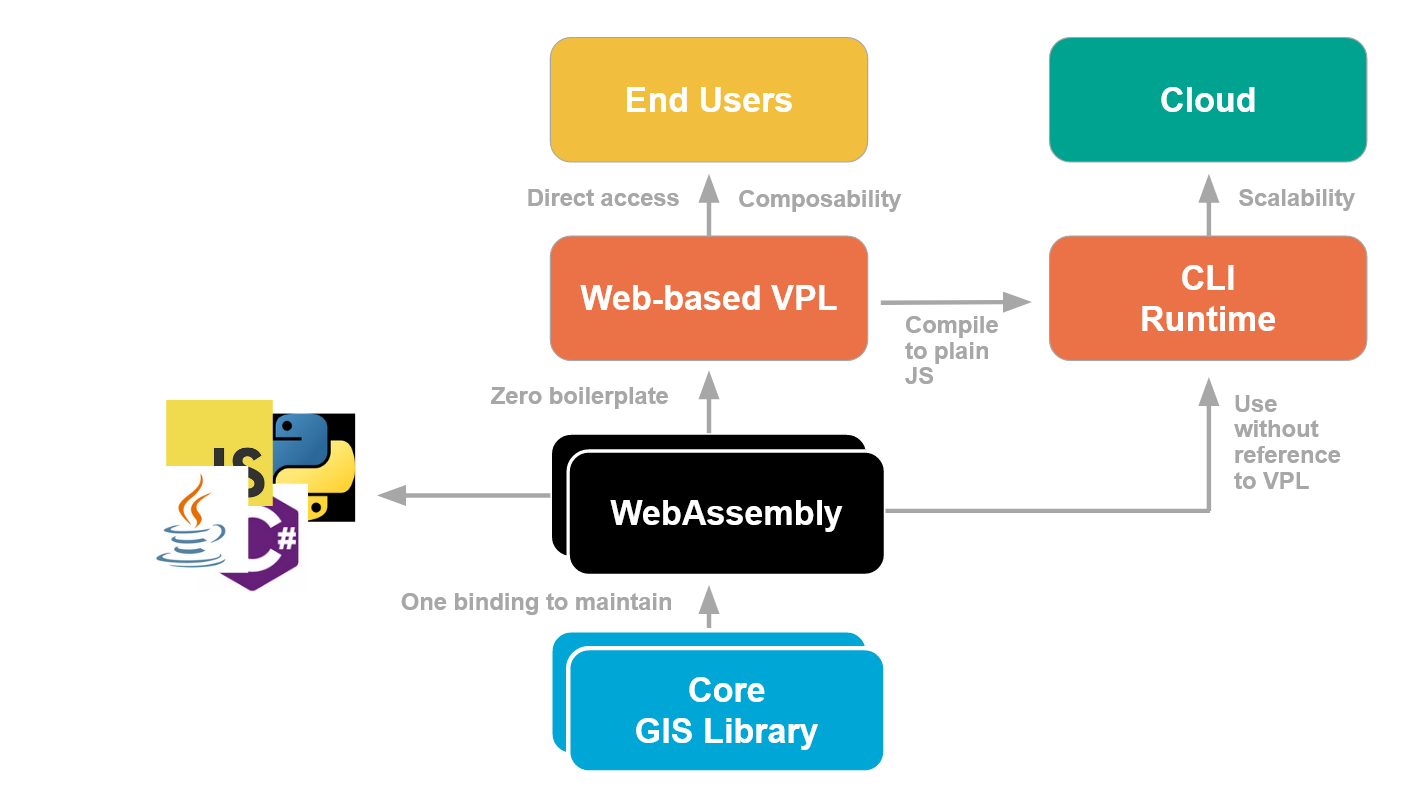
\includegraphics[width=\linewidth]{expanded-proposal.png}
  \end{subfigure}%
  \caption{An expanded proposed methodology, to provide a backend, cloud-based execution}
  \label{fig:proposal-extended-again}
\end{figure}

\begin{figure}
  \centering
  \graphicspath{ {../../assets/images/implementation/} }
  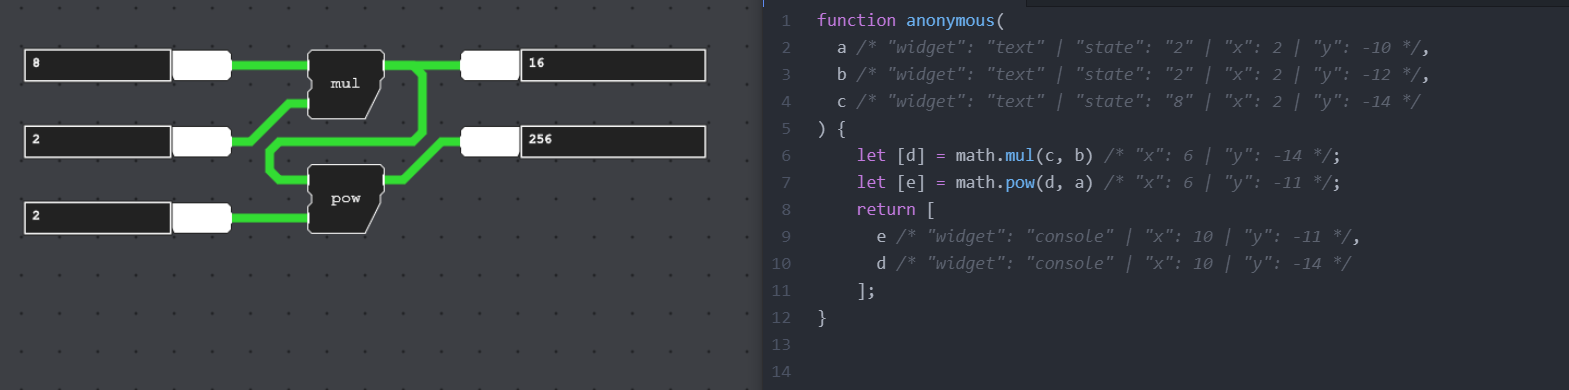
\includegraphics[width=\linewidth]{early-geofront.png}
  \caption[Geofront to js]{An early build of geofront, showing compilation to javascript}
  \label{fig:early-geofront-compile-to-js}
\end{figure}

An early build of Geofront had the ability to compile a Geofront script to regular javascript (see (\reffig{fig:early-geofront-compile-to-js})).  
All libraries were converted to normal import statement, all nodes were replaced by function calls, and the cables substituted by a variable token. 
This way, the application could be run headless (without the \ac{GUI}) either the browser or on a server, using a local javascript runtime like Deno \citep{contributors_deno_2022}.

A future study could re-implement this feature, opening up the possibility for deployment and scalability: 
Scripts created with geofront could then deployed as a web worker, as a web applications of themselves, or as a web processing services \citep{open_geospatial_consortium_web_2015}.
Also, by running this script on a server, and ideally a server containing the geodata required in the process, one could deploy and run a Geofront scripts on a massive scale. 

The overall purpose of this would be to create a \ac{FOSS} alternative to tools like the Google Earth Engine, and FME cloud compute. 

\subsection{Streamed, on demand geocomputation}

This study showed that browser-based geocomputation is reasonably viable. 
This might allow for a new type of geoprocessing workflow, which could replace some use-cases that now require big-data processing and storage.
A big problem in the \ac{GIS} industry is having to process and store sizable datasets, while only a portion of it will be actually used. 
A possible solution could be to take a raw dataset base layer, and process it on-demand in a browser.

This would have several advantages. 
First, end-users can specify the scope and parameters of this process, making the data immediately fine-tuned to the specific needs of this user. 
Secondly, this could be a more cost-effective method, as cloud computation \& Terabytes of storage are time consuming and expensive phenomena.

This type of \emph{on demand geocomputation} is certainly not a drop-in replacement for all use cases. 
But, in situations which can guarantee a 'local correctness', and if the scope asked by the used is not too large, this should be possible. 
Examples of this would be a streamed delaunay triangulation, TIN interpolation or color-band arithmetic. 

\subsection{Rust-based geocomputation \& cloud native geospatial}

An interesting aspect this study was able to touch on is using Rust for geocomputation.
The reason for this was the extensive support for webassembly, which was essential for browser-based geocomputation. 
However, there are additional reasons one might want to perform geocomputation within Rust.
One is that rust is widely considered as a more stable, less runtime error-prone language than C++, while offering similar performance and features.
Additionally, rust Wasm binaries also tend to be smaller than C++ wasm binaries.  

This could be very interesting to the "cloud-native geospatial" movement. 
This \ac{GIS} movement aims to create the tools necessary to send geocomputation to servers, rather than sending geodata to the places where they are processed.
To do this, geocomputation must become more portable than it currently is, and Rust compiled to WebAssembly might proof to be a strong candidate for creating exchangeable, performant, compact, and error-proof binaries.
It already sees usage on both cloud and edge servers (State of WebAssembly, 2022).  

Therefore, studying Rust-based geocomputation for the purpose of cloud native and edge computing, would be a promising topic for subsequent research. 

\subsection{FAIR geocomputation}

% The study has only scratched the surface on what is possible with combining geocomputation with the fields of Visual programming, and web applications. 
The introduction theorized on how both VPLS and web-apps could be used to make geocomputation less cumbersome.
The study chose to pursuit this on a practical, technical level. 

However, a more theoretical study could also be performed. 
It turns out that these ideas of 'less cumbersome geodata processing', have something in common with many of the geoweb studies on data accessibility and usability \citep{brink_geospatial_2018}.
The ideas of 'data silo's', 'FAIR geodata', and 'denichifying of \ac{GIS} data' (see \citet{brink_geospatial_2018}) map well to geocomputation:
Functionality Silo's, FAIR geocomputation, denichifying of \ac{GIS} computation. 

Therefore, an interesting question for a subsequent study could be: "How could geocomputation become more Findable, Accessible, Interoperable, and Reusable?", or "How to integrate the function-silo's of GIS, BIM \& CAD?"
By focussing on data processing actions rather than the data itself, we could shed a new light on why data discrepancies and inaccessibility exist. 
After all, if a user is unable to convert retrieved geodata to their particular use case, then the information they seek remains inaccessible.


% \subsection*{Reproducibility}
% This section provides a discussion on the reproducibility of the developed methods and obtained results in this study.


% \subsection{Hybrid geocomputation}

% Lastly, 


  
  % Sub component: FAIR: 
  % - FINDABLE:      Hard to find the right tools for the job
  % - ACCESSIBLE:    Hard to access these tools (install, setup environment, look at what you are doing)
  % - INTEROPERABLE: Hard to use two tools from different ecosystems (bindings, plugins, etc). 
  % - REUSABLE:      Hard to re-use a specific scripts written for one use case in another use case

% (NOTE: This is a nice point to make after the thesis: focus more on FAIR geoprocessing)

% The Geoweb, or Geospatial Web, covers a broad collection of topics located at intersection of the field of geo-information and the web. A noteworthy study on the Geoweb is Van den Brink's phd titled "Geospatial Data on the Web". \cite{brink_geospatial_2018}. She claims that even though geodata is vital to a diverse range of applications and people, the ability to properly retrieve geodata remains almost exclusive to experts in the field. This is to the determent of all these applications and people, jeopardizing value, opportunity, and decision making. She makes this argument by using the concept of FAIR geodata. Coined by \cite{mark_d_wilkinson_fair_2016}, The FAIR principles are a collection of four assessment criteria used to judge the usability of (scientific) data: Findable, Accessible, Interoperable, and Reusable. 

% We argue that if these concerns count for geodata \textit{retrieval}, they should just as well count for geodata \textit{processing}. After all, if a user is unable to convert the retrieved geodata to their particular use case, then the information they seek remains inaccessible. Therefore, this study introduces the concept of \emph{FAIR geoprocessing}. 

% Based on the arguments presented by \cite{brink_geospatial_2018}, we can also extrapolate that a \ac{gis} environment shouldn't exclusively be used by only experts. Van den Brink mentions a group called 'data users', presented as "web developers, data journalists etc. who use different kinds of data, including geospatial data, directly to create applications or visualizations that supply information to end users (citizens)". 

% We use both extrapolations to define the users and 'usability' for the context of this study. We will judge the proposed use case application as 'usable', if it is deemed Findable, Accessible, Interoperable, and Reusable. The user group intended to use this environment is defined as both experts in the field of geo-information and this more general group of data users.

% Function Silo's \& denichification of GIS

% similarly: function silo's 

% / experiment to assess: 
% - The fitness of the web in general for client-side geo-computation
% - If new features of modern browsers mean anything for the field of geo-informatics at large 
% - The topic of accessible geoprocessing.

% now, answer this to the best of your ability

% Many considerations

% Premature optimization is the root of all evil | Donald Knuth
% Delay decisions to the latest moments, to gain maximum context,
% Key insight into writing better compilers

% While conducting this research, I came across various key insights from various studies, and there seemed to be a link between them 

% Most important effort I saw is the "denichification" of the geospatial world.
% - Hugo's keynote
% - Linda van den Brink's PHD
% - cloud-native geospatial 

% We focus on Access

% \m{->} the fact of being able to be reached or obtained easily:
% \textit{Two new roads are being built to increase accessibility to the town centre.}

% \m{->} the quality of being easy to understand: 
% \textit{The accessibility of her plays means that she is able to reach a wide audience.}


%%%%%%%%%%%%%%%%%%%%%%%%%%%%%%%%%%%%%%%%%%%%%%%%%%%%%%%%%%%%%%%%%%%%%%%%%%%%%%%
%%%%%%%%%%%%%%%%%%%%%%%%%%%%%%%%%%%%%%%%%%%%%%%%%%%%%%%%%%%%%%%%%%%%%%%%%%%%%%%
%%%%%%%%%%%%%%%%%%%%%%%%%%%%%%%%%%%%%%%%%%%%%%%%%%%%%%%%%%%%%%%%%%%%%%%%%%%%%%%


% \subsection{Cloud Native}
% Lastly, the 

% - The front-end browser technologies are a vital component of the modern geospatial software.
% - Like how the entire cloud-native moment is only possible because of the HTTP range request feature. 

% - a vital component of the cloud-native geospatial moment is the "HTTP range request" web feature, and chris said as much.
%   - this feature has been out for some time ( html1/1, )
% - What I'm saying, is that we have a whole range of similar, 'game changing technologies' recently added to web browsers, and I have a feeling these features could be the birthing grounds for new, ground breaking ideas and movements of ideas. 

% We have not fully envisioned these new trends, nor do we have a catchy, powerful name such as \emph{Cloud Native Geospatial}, But I have no doubt that something revolutionary will come of this. 

% Nevertheless, I will attempt to name and envision a trend from these technologies. \emph{"FAIR Geodata Processing"}.

% Vision: 
% - Portable, cross-platform, binary geoprocessing libraries, which can be used on the cloud / on servers, natively, and in the browser, without any changes. 
% \m{->} we can use that to build standards for geodata processing itself. Every \m{GP} library interoperable with every other library, at least on a language and package manager level.
% - This also eliminates the need of platform specific plugins (QGIS plugins, ARCGIS plugins, Blender Plugins, 'web plugins').
% - This could lead to a generalized geoprocessing library portal like NPM / cargo / WAPM with an attached content delivery network, Or these infrastructures can just be utilized, with just an UI sprayed on top.

% - I am aware that these types of efforts have been attempted many times before, but WebAssembly might be a missing link 

% \m{->} webassembly has a good balance between portability and performance.

% \m{->}

% If I were to attempt to name this trend, I would


% \begin{note}
  
% recommendations: 
% - go native, since it is better suited for these types of applications
%   - native VPL 
%   - use a native GUI library
% \end{note}

\section{Reflection}
\label{sec:reflection}

Here I reflect on possible shortcomings of the thesis in terms of value and quality, and how I have attempted to address these shortcomings. 

\textbf{Biases regarding C++ and Rust}

First of all, in the comparison between C++ and Rust, the studies conducted proved to be unfavorable towards C++. 
it could be that C++ was judged unfairly, due to the authors personal inexperience with the build tooling of the language. 
Many complications were encountered during compilation, leading to extensive editing of makefiles and attempts at recompiling forked subdependencies of CGAL using 'hacky fixes'.  
It is unknown how much of this was due to personal C++ inexperience, inflexibility of the libraries in question, or the shortcomings of the toolchain. 

Despite this, the study performed steps to make the judgement as non-biased as possible.
Preliminary studies were conducted with both languages, and additional C++ courses were followed. 

It could even be the case that this particular study is more fair than a study conducted by authors with more experience with C++, 
since before the assessment between Rust and C++, approximately the same amount of time was spent with both languages. 

\textbf{Scope too wide}

Additionally, the scope generated by combining geocomputation, web applications and VPLs, might have been too extensive. 
This is evident in the number of 'supporting studies' conducted, and the sizable workload of the implementation.
A better approach might have been to focus the scope of the thesis down to only 'browser-based geocomputation', or 'visual programming and geo-computation', or 'geocomputation using rust', to allow for a more in-depth analysis.

On the other side, the core of the contribution of this thesis lies precisely in the attempt to connect these subjects,
especially since prior studies remained by en large closely scoped to their respective domains.
The hypothesis was that a certain synergy may exist, and that each separate domain stand to gain from the ideas and knowledge found in the other ones. 
In order to make this possible, the study had to acquire a scope to explore all in-between synergies and interactions, leading to geo-vpls, web-vpls, and browser-based geocomputation. 
Now that this study has made these connections explicit, future studies can focus on more precise aspects of these cornerstones again.

\textbf{Too distant from the field of GIS}

Where the exact boundary of one field of study is, and where another begins, remains of course a fuzzy question. 
Still, the direction of this study appears to stray far from 'core GIS concerns', and appears more in one line with the  field of "End User Development (EUD)", and fields like "Computer-Human interactions". 

In defense of this, the field of GIS, like all research, is built on top of more foundational work which came before it. 
However, during the implementation of the study, it appeared that little foundation was in place for a geo-web-vpl specifically. 
This made it necessary to generalize, to build the missing foundation first.
For example "How can \emph{any} library be compiled and loaded into \emph{any} web-vpl" is a question which had to be answered first. 
Then, the question could be specified to \emph{geometry} and \emph{geo-web-vpl}. 
And only after that, the geodata and geoprocessing libraries specific to the field of GIS could be regarded. 
By doing so, this study wishes to provide a foundation to assist any subsequent future study in this direction, which can then be more GIS focussed.

% \textbf{Imbalance between software implementation and study}

% The fourth 'danger' which remained an ongoing balancing act during the execution of this study, is the balance between 'performing a study' and 'developing an application'. 
% Indeed, many of the aspects discussed throughout this study come down to implementation aspects of the geofront application. 

% PROBLEM: WHAT DO I TEST??

% This is why the study has attempted to generalized its findings as much as possible.
% Geofront is regarded as a proxy of geo-web-VPLS in general, in the sense that whatever was encountered during implementation of the application, must be the same for any attempt at creating a web-based vpl for geocomputation.


\textbf{Subjectivity in qualitative assessment}

Lastly, many of the assessments made by this study are qualitative assessment, and as such, might suffer from a high level of subjectivity. 
This is unavoidable in any assessment which does not come down to clear, quantifiable aspects, such as performance, memory usage or precision. 

Nevertheless, the study has attempted to scope this subjectivity by basing its assessments heavily on prior works in the field of vpl, and always showcasing clear examples. 

% \section{Personal Reflection}
% \label{sec:personal-reflection}

% A thesis is, among many things, an attempt to formulate. 
% To clarify and structure a phenomenon, as much for yourself as for the public. 
% This thesis can also be regarded as such an attempt. 
% I tried to understand a phenomenon you might call: "End User Geodata Processing". 
% To what extent can the activity of geocomputation truly be made "publicly available", besides writing open source software?
% I see this in much similar terms to the "Teach a man how to fish..." saying.
% Providing open geodata to the public is great, but we might only be "Giving a man a fish so he can eat for a day".
% By providing geocomputation tools in a fashion usable by end users, we could give the general public more authorship and autonomy over geodata. 
% And, more concretely, if a person themselves can compute what they want, when they want it, we don't have to pre-process several variants of the same dataset, tweaked to suit different audiences, saving storage and especially processing time.

% I did not have this clear of a goal at the start of the thesis, only intuitions and a set of loosely coupled ideas.
% I was also unable to find a foundational body of work to base this research on. 
% What I did know is that I did not want to stay at a theoretical level. 
% I wanted to truly \textbf{build} a solution, to the at this point ill-defined problem. 

% In hindsight, I don't think it was wise to build a concrete software implementation based on multiple, loosely defined theories. 
% This imbalance led to a time-consuming complication between research and software implementation while writing the thesis.

% Nevertheless, through many iterations, I was eventually able to integrate both the ideas and the thesis at large with this software implementation.
% I have learned two additional major lessons from conducting this study: 
% One, writing well is hard work. 
% Boiling a story down to the essentials asks a great deal of time and energy. 
% I would not call the current story this study tells concise, but it is much more precise than I was able to write at the beginning of this adventure.

% And two, I must learn to rely on the work of others.
% This is difficult, as it is contrary to my personal conviction on the great importance of "learning from scratch".
% Both the software implementation and the written thesis had me figuring out a lot of aspects from scratch, and this had advantages and disadvantages.
% The advantage is that 'doing the work again yourself', is probably one of the most educational endeavors one can do. 
% We must understand the inner workings of the systems we work with, and especially of the systems we wish to improve. 
 
% This is why I took the risk of developing many aspects of this thesis anew. 
% Even if this might turn out to be a parallel study, it would only reinforce the 're' in research. 

% The disadvantage of doing this, is that you prevent yourself from being able to 'stand on the shoulders of giants'.
% I especially felt the sting of this lesson in the written aspect of this thesis. 
% Not really knowing up from down because of having no readily available work to build on caused countless hours of revision.
% Another great disadvantage is that you run the risk of alienating both yourself and your endeavors. 
% By building from existing starting points, you connect your work with the works of others, and in doing so contributing to a wider community.

% If you have read this thesis up to this point, I want to sincerely thank you for your time and interest.
% With this thesis, I hope to have provided you and the wider geospatial community with something of value.

% \section{Personal Reflection}

% One of the goals of this study was to investigate and explore browser-based geo-computation, and there are many ways of conducting exploitive studies. 
% This study chose for a practical approach: investigation by means of creating an application.
% The advantage of this approach is that it leads to tangible results. 

% The disadvantage of this approach is that software development can lead a study astray, if the development needs of the application are put before the needs of the study itself.

% This study was a battleground between "performing a study on if geocomputation benefits from the web \& a vpl", and "lets build an open-source tool to aid geocomputation"

% It needed a bit of both.


% \begin{note}
  
%   Reflection
  
%   "It is not the task of the University to offer what society asks for, but to give what society needs" ~ Edsger W. Dijkstra
  
%   Despite the cliche of quoting Dijkstra, and despite the arrogant danger of pretending to know what people want better than they themselves know what they want, 
  
  
%   'what the world wants is more react, angular, or vue developers'
%   'what the world needs, in my opinion, is guidance on this front of web vs native application development.'
  
%   right now, we are sucked in the rabbit hole of 'make everything web-based, then maybe try to execute that natively',
%   And I think that we should start working towards a situation of: 'make everything natively, KNOWING that publishing it on the web is a piece of cake'.
  
  
  
%   The thesis represents to me a bold "What if" scenario: 
%   - What if geodata computation was an elegant, ergonomic process?
%   - What if more people could more easily perform geospatial computations?
%   - What if textual and visual programming languages worked complimentary?    
%   - What if geocomputation libraries where written in Rust instead of C/C++?
%   - 
  
%   'we are not inventive enough with the tools at our disposal'
%   'outdated web vs native, client vs server distinctions block our vision from seeing new types of applications'
%   'we could be doing so much more with what we have.'
  
  
%   A huge leap 
  
  
% \end{note}
  
%   \subsection{Personal Motivation}
%   During my internship I was tasked with creating a parametric 3D CAD model. 
  
%   - local usage 
%     -> quick, direct feedback
  
%   - We needed to make this a product for end users. 
  
%   - Industry-standard choice: cloud 
%     -> smart-server dumb-client setup, cloud-native architecture 
  
%   - Problems
%     -> continuously downloading new resulting CAD files after every change created a lot of web traffic. 
%     -> slow, not at all the same experience.
%     -> cloud host was even more slow in cold-start scenario's   
%     -> cloud host monetization scheme: pay for every time the script runs, 
%        -> meant that consumers had to be discouraged to 'play around' with the tool too much. 
    
%   This made me question the cloud-based paradigm, at least for the use case of calculating geometry by end users. 
  
%   At the same time, many of our parametric designers could use grasshopper, and only grasshopper. 
  
%   This led me to think about a vpl which can run client-side in a browser, and can produce client-side applications.
  
%   if the data is geodata or CAD data, does not matter besides the fact that geodata is often big data.
  
  

%   \textbf{Motivation 2: Accessible Geoprocessing Libraries}
  
%   Most industry-standard geoprocessing libraries such as CGAL are difficult to use by anyone but experts in the field. A steep learning curve combined with relatively complex installation procedures hinders quick experimentation, demonstration, and widespread utilization of these powerful tools. It also limits the interdisciplinary exchange of knowledge, and compromises the return of investment the general public may expect of publicly funded research.
  
%   Geofront could improve the accessibility of existing geodata processing and analysis libraries, without adding major changes to those tools, by loading webassembly-compiled versions of them, similar to [other web demo's](todo).

% \subsection{Reproducibility}

% Results themselves are insanely reproducable.
% Software can be used, you can reproduce results easely by dumping versions of geofront in 
% a folder.

% \dots

% Software can also be build without too many difficulties, but the procedure has some unconventional build steps: 

% \dots

% BUT, the code is not the cleanest, nor the most conventional. minus points on open-source accessibility.

%%%%%%%%%%%%%%%%%%%%%%%%%%%%%%%%%%%%%%%%%%%%%%%%%%%%%%%%%%%%%%%%%%%%%%%%%%%%%%%
%%%%%%%%%%%%%%%%%%%%%%%%%%%%%%%%%%%%%%%%%%%%%%%%%%%%%%%%%%%%%%%%%%%%%%%%%%%%%%%
%%%%%%%%%%%%%%%%%%%%%%%%%%%%%%%%%%%%%%%%%%%%%%%%%%%%%%%%%%%%%%%%%%%%%%%%%%%%%%%

% \section{Self Assessment}

% \subsection{Using Geofront for CAD or BIM}

% \todo{make it more nuanced}
% % AT THE END OF THE DAY, THERE IS NO REAL DIFFERENCE BETWEEN CAD, BIM and GIS.
% % of course, there are many differences, like required precision and tolerances, which types of interfaces and operations are common, and the subject matter it represents. 
% % But on a deeper, fundamental level, they are all the same: its just a bunch of 2D / 3D data, representing some real world thing. 

% Today, we see the need for collaboration between CAD, BIM and GIS. Entire industries (Speckle, FME) have been introduced to bridge the gaps. 

% All three of CAD, BIM and GIS want the ability to join solids together, desire to give certain spatial objects metadata, and want to run automated workflows in the cloud. These Individual fields are constantly reinventing features the other fields have already figured out. BIM is starting to open up to the idea of streaming only a part of the building instead of the whole thing, something which the GIS world has been doing for years. On the other hand, GIS is only now starting to make the transition to 3D, a transition not unlike to how BIM is replacing 2D CAD in the AEC industry. 

% We will allow geofront to be fully customized by different plugins. By unloading all GIS plugins, and adding all BIM plugins, we turn GeoFront from a GIS to a BIM tool.









% In one sentence: It was my goal to make your grandma use CGAL.
% This requires making something extremely user-friendly compared to QGIS / python (the vpl)
% As well as making it extremely accessible (wasm: no install, direct usage)




\chapter{Post-Conclusion}%%%%%%%%%%%%%%%%%%%%%%%%%%%%%%%%%%%%%%%%%%%%%%%%%%%%%%%%%%% CHAPTER

\section{On the future}

This study was ....

The study was performed for many reasons

Many considerations



\subsection{Use Cases of Browser Based Geoprocessing}



- For which use-cases might such an application be beneficial? (~Old Phase 4)
- Name all reasons for browser based geoprocessing, and the 4 audiences.

Discuss 

\section{Reproducibility}
% This chapter explains how this thesis might be reproduced, as well as 

Reproducibility
Results themselves are insanely reproducable.
Software can be used, you can reproduce results easely by dumping versions of geofront in 
a folder.

\dots

Software can also be build without too many difficulties, but the procedure has some unconventional build steps: 

\dots

BUT, the code is not the cleanest, nor the most conventional. minus points on open-source accessibility.



\subsection{Environment}%%%%%%%%%%% SECTION
- github organization 
- repo for engine 
- repo for app 
- repo for each plugin
- build procedure

\subsection{Usage}%%%%%%%%%%% SECTION

\emph{basically, write a tutorial}

This is how one can use Geofront

\subsection{Creating \& Using your own code}
\emph{show the insane (rust + wasm + npm) workflow}

Locally: 
1. Write a geoprocessing / analysis library using a system-level language (rust, C++).
2. Expose certain functions as public, using 'wasm-pack' or 'emscripten'.
3. Compile to `.wasm` + `d.ts` + `.js`.
4. publish to npm (very easy to do with wasm-pack, can also be done with emscripten)

Alternatively: 
1. Write a library using typescript, 
3. Compile to `d.ts` + `.js`.
4. publish to npm 

In Geofront: 
4. Reference the CDN (content delivery network) address of this node package. 

Congrats, this is now a publicly accessible geofront plugin!
The library is loaded, A component is created for each function, with inputs for input parameters, and a singular output. If a 'typescript tuple type' is exported, the plugin loader will create multiple outputs according to each component of the tuple.

\section{Limitations}%%%%%%%%%%% SECTION

Limitations of usage right now



\section{Future Work}
Boulevard of broken dreams :) 

This thesis has only scratched the surface of all that

- Geofront as web-based version of grasshopper
- Geofront as lightweight QGIS replacement 



\appendix

%%%
\cleardoublepage
%-- *mandatory* appendix about the reproducibility


\chapter{Reproducibility self-assessment}

\section{Marks for each of the criteria}

\begin{figure}[h]
  \centering
  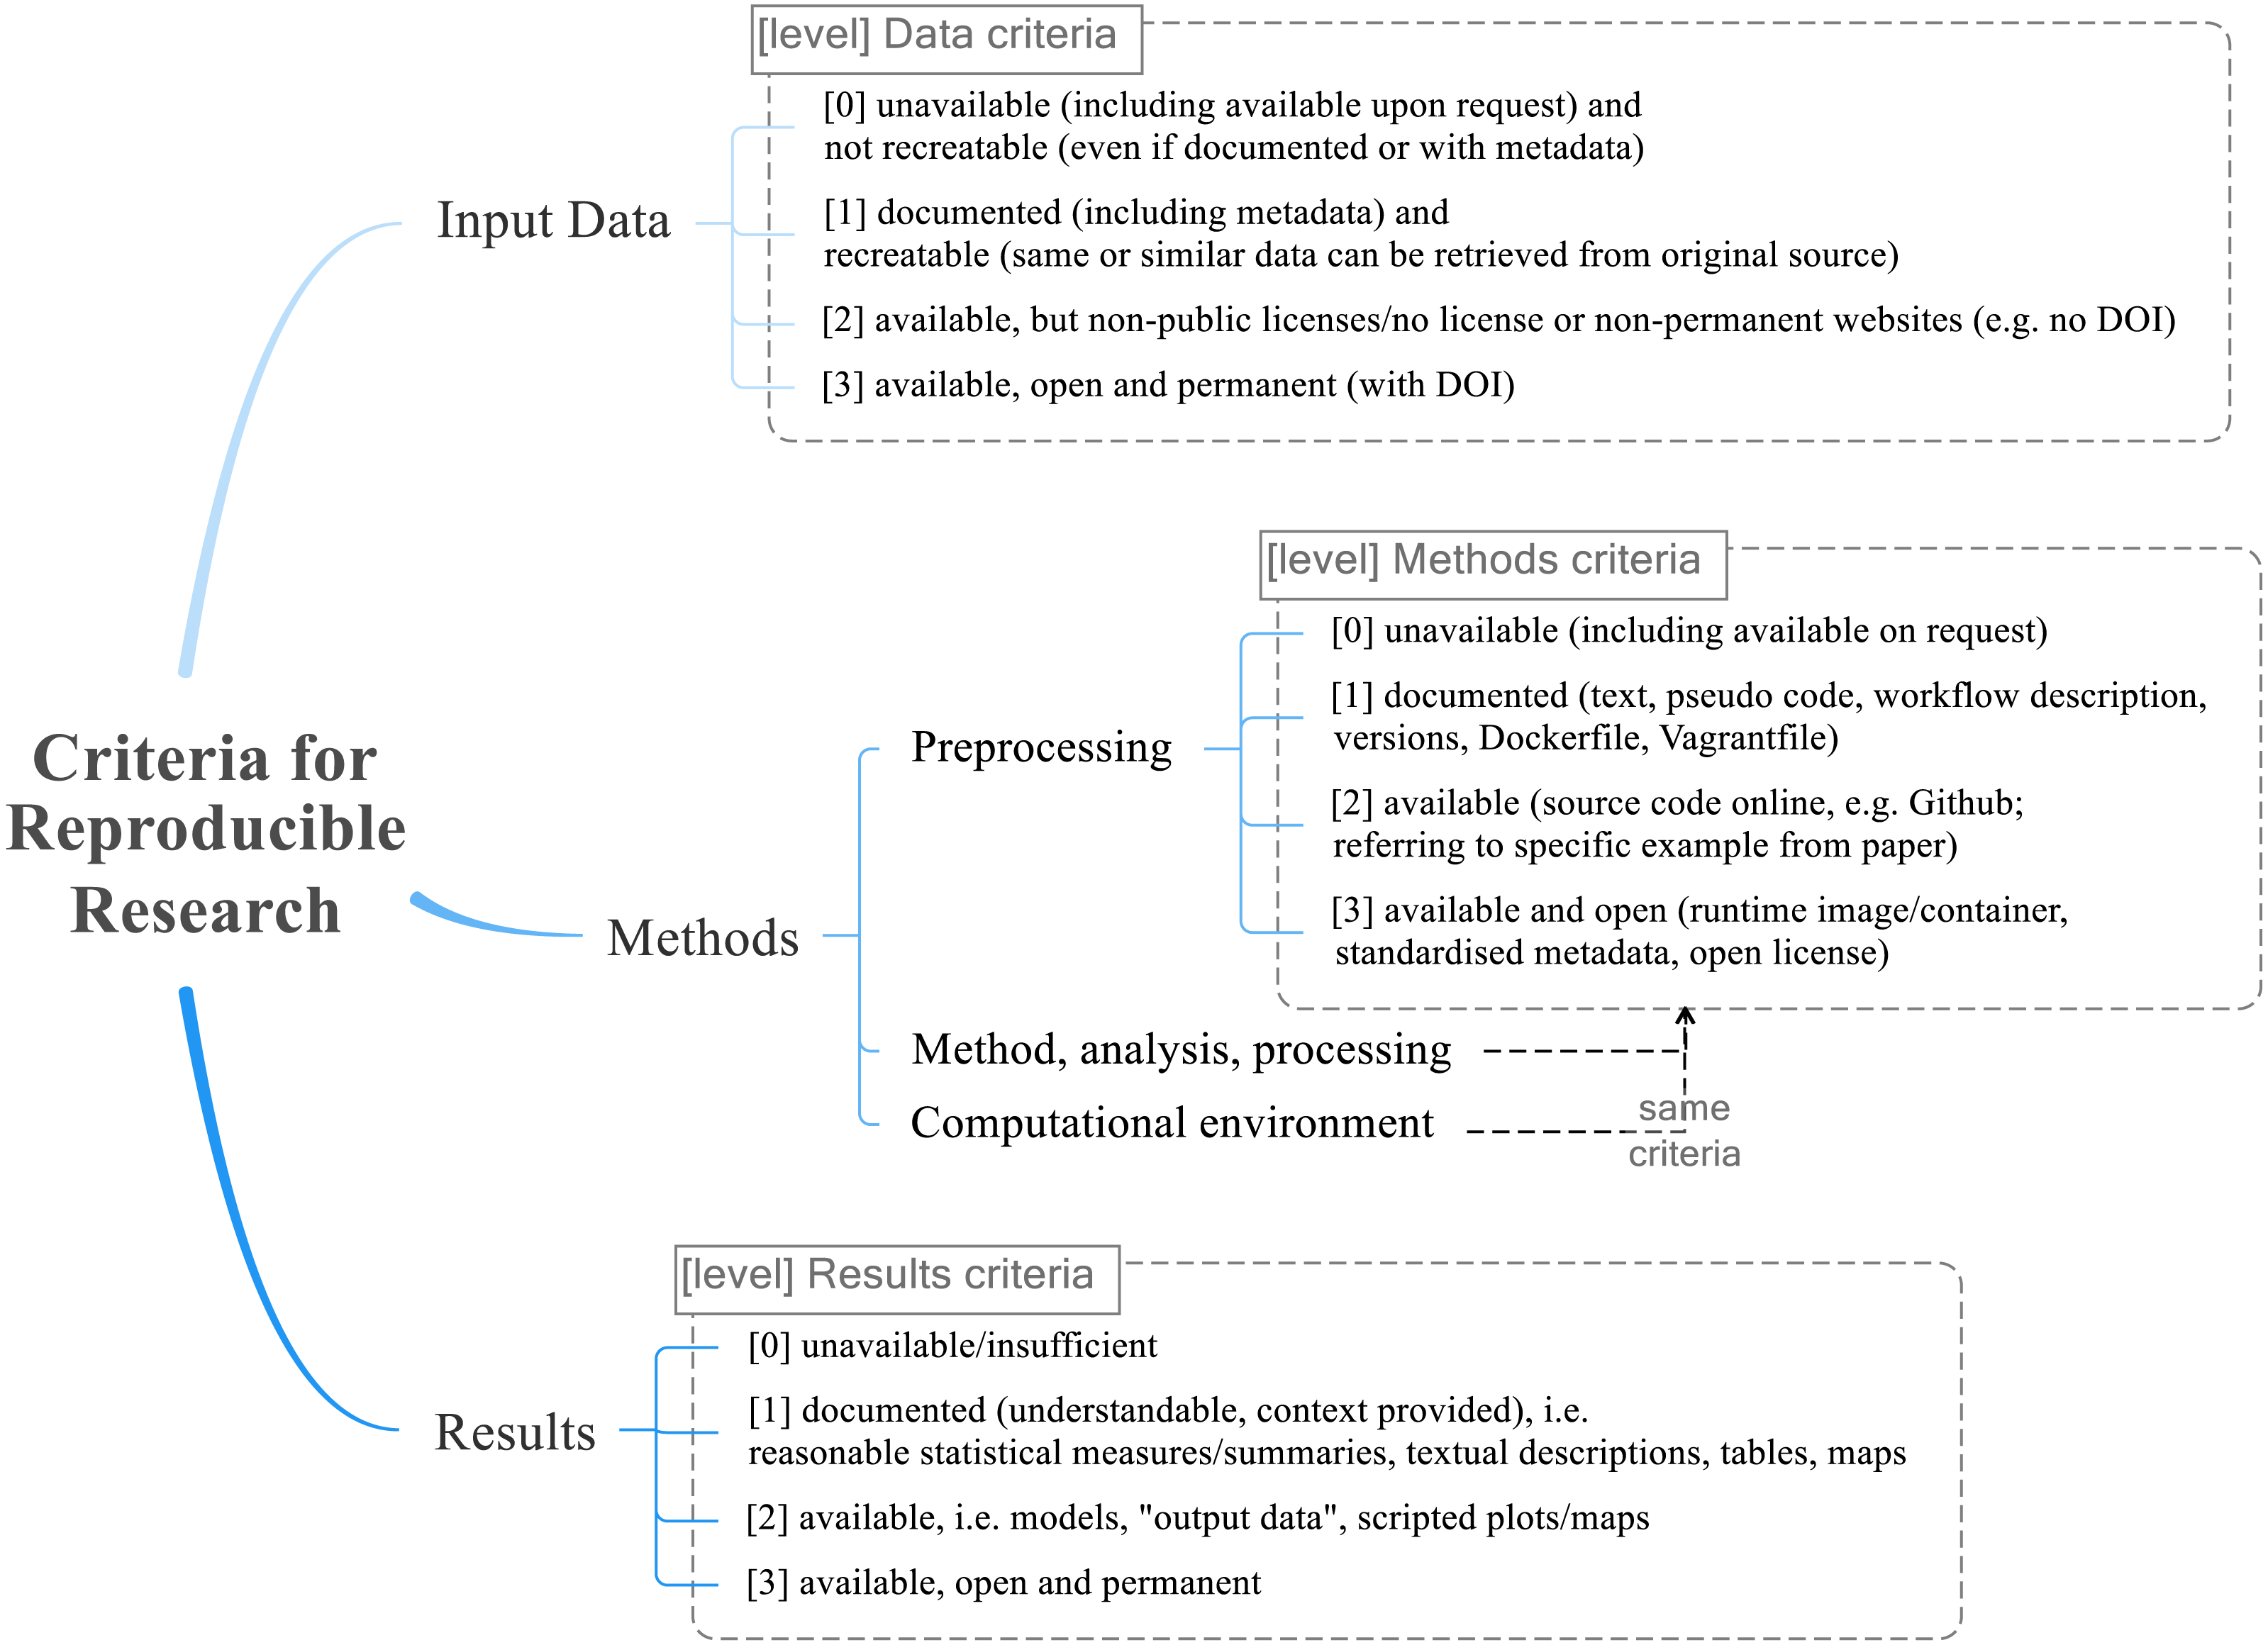
\includegraphics[width=0.8\linewidth]{figs/reproducibility_criteria.png}
  \caption{Reproducibility criteria to be assessed.}
\label{fig:reproducibility_criteria}
\end{figure}

Grade/evaluate yourself for the 5 criteria (giving 0/1/2/3 for each):
\begin{enumerate}
  \item input data
  \item preprocessing
  \item methods
  \item computational environment
  \item results
\end{enumerate}


%%%
\section{Self-reflection} 

A self-reflection about the reproducibility of your thesis/results.

We expect maximum 1 page here.

For example, if your data are not made publicly available, you need to justify it why (perhaps the company prevented you from doing this).

%-- other examples of Appendix, not mandatory


\chapter{Some UML diagrams}

\begin{figure}
  \centering
  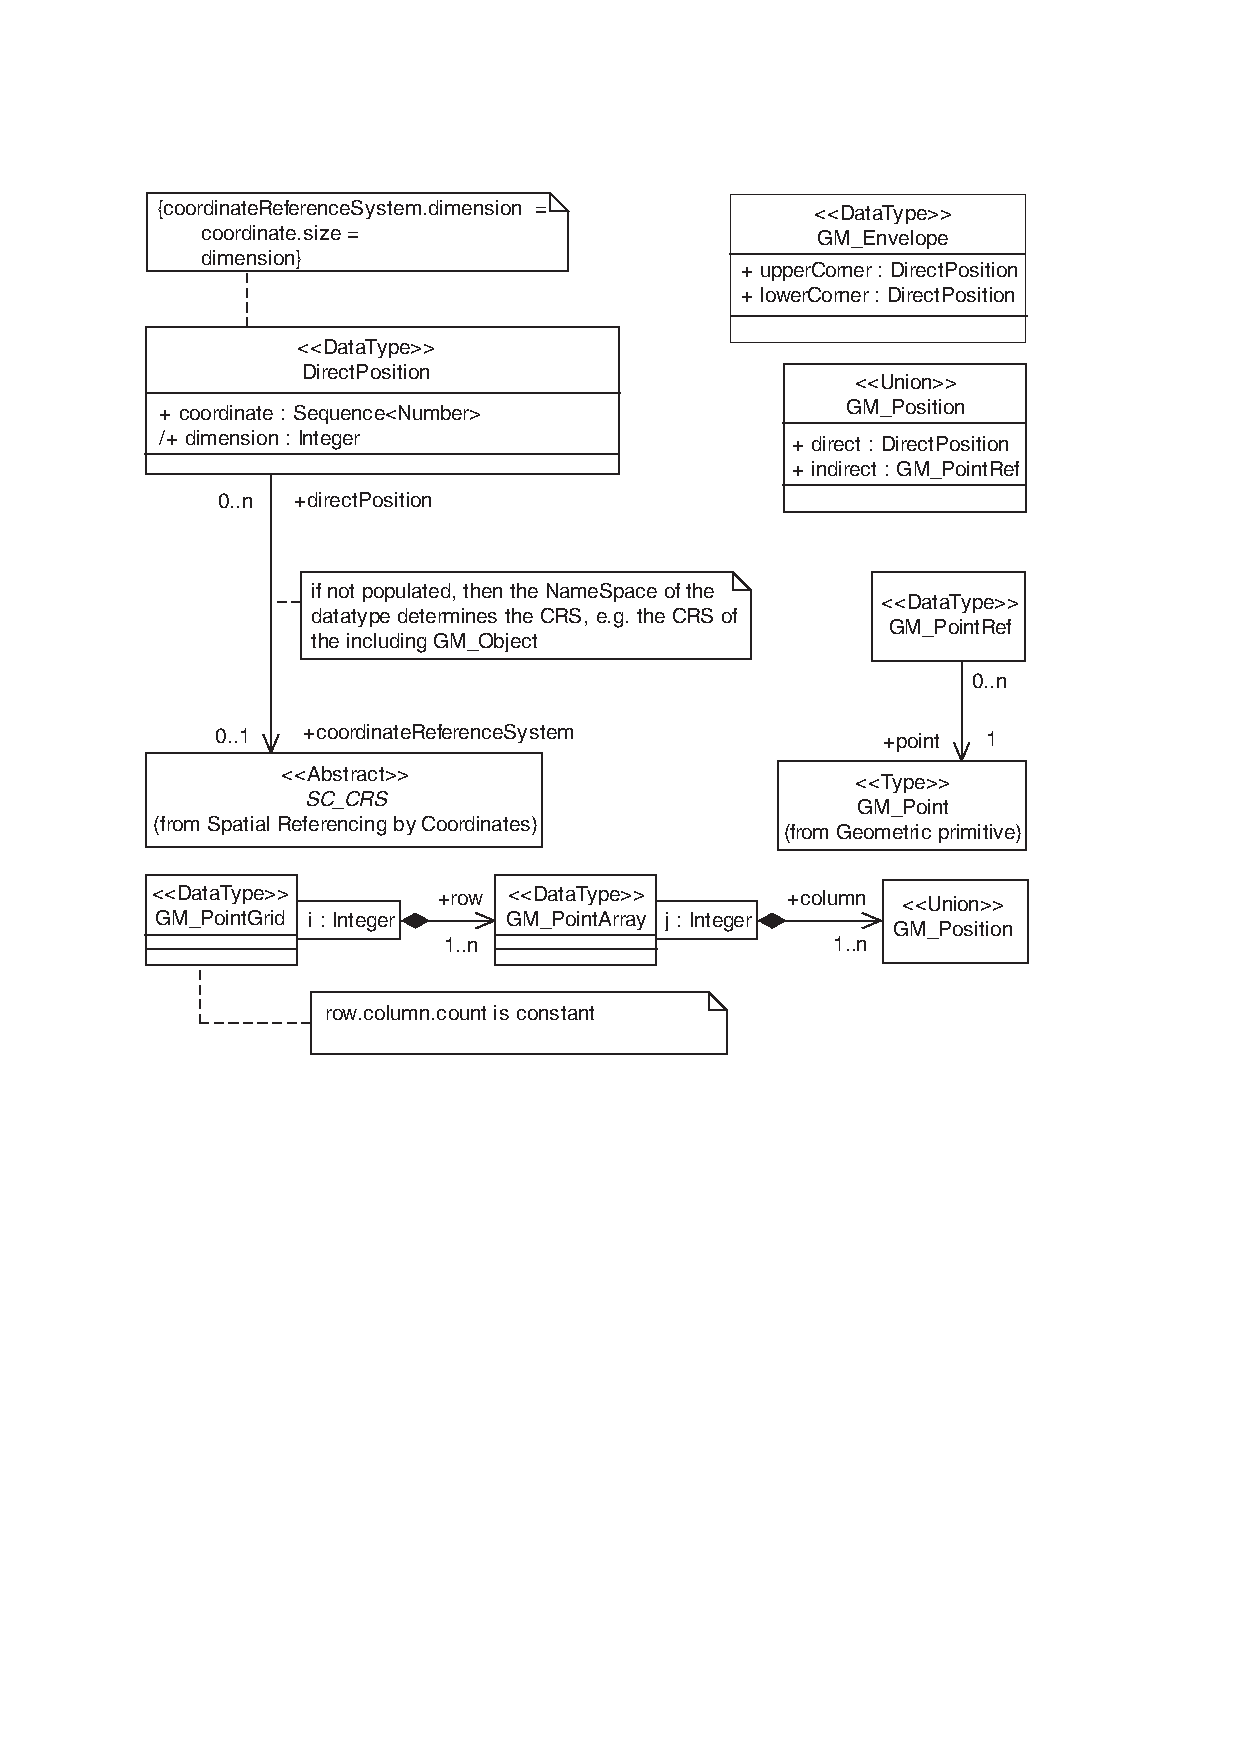
\includegraphics[width=0.8\linewidth]{figs/someuml.pdf}
  \caption{The UML diagram of something that looks important.}
\label{fig:someuml}
\end{figure}

% *****************************************************************
% Backmatter
%******************************************************************
\backmatter 

%- bibliography
\bibliographystyle{apalike}
\bibliography{library}



\clearpage
%*******************************************************
% Colophon
%*******************************************************
\thispagestyle{empty}

\hfill{}
\vfill{}

\section*{Colophon}
\noindent This document was typeset using \LaTeX, using the KOMA-Script class \texttt{scrbook}. The main font is Palatino.
% The figures and diagrams were mostly drawn using IPE, PGF/Ti\emph{k}z and Omnigraffle. 


\cleardoublepage



\includepdf{0-cover/cover_back.pdf}

\end{document}





